\documentclass[conference]{IEEEtran}
\IEEEoverridecommandlockouts
\usepackage[utf8]{inputenc}
\usepackage[spanish]{babel}
\usepackage{cite}
\usepackage{amsmath,amssymb,amsfonts}
\usepackage{algorithmic}
\usepackage{graphicx}
\usepackage{textcomp}
\usepackage{xcolor}
\def\BibTeX{{\rm B\kern-.05em{\sc i\kern-.025em b}\kern-.08em
    T\kern-.1667em\lower.7ex\hbox{E}\kern-.125emX}}
\begin{document}

\title{Métodos de Gradiente Proximal para Optimización Dispersa en el Análisis de Calidad del Aire PM2.5 del Área Metropolitana de Lima}

\author{\IEEEauthorblockN{Carlos Paolo Fontanil Barrera}
\IEEEauthorblockA{\textit{Facultad de Ingeniería Estadística} \\
\textit{e Informática}\\
\textit{Universidad Nacional del Altiplano}\\
Puno, Perú \\
fontanilbarreracarlospaolo@gmail.com}
}

\maketitle

\begin{abstract}
Air pollution monitoring, particularly fine particulate matter (PM2.5), presents significant computational challenges requiring advanced optimization techniques. This paper proposes the application of proximal gradient methods for sparse optimization in PM2.5 concentration analysis within Lima Metropolitan Area. We implement a Fast Iterative Shrinkage-Thresholding Algorithm (FISTA) combined with LASSO regularization to identify key temporal and environmental predictors from a comprehensive 10-year dataset (2015-2024). The sparse optimization framework automatically selects relevant features while maintaining prediction accuracy. Our methodology achieved R² = 0.847 with RMSE = 4.23 μg/m³ using only 8 out of 15 engineered features. Key findings include strong temporal persistence (PM2.5 at t-1, t-6h), seasonal patterns, and rush-hour indicators as primary predictors. PM2.5 concentrations exceeded WHO guidelines (15 μg/m³) in 68.4\% of measurements and Peru's Environmental Quality Standards (50 μg/m³) in 23.7\% of cases. The proximal gradient approach demonstrates superior convergence properties and interpretability compared to traditional methods, providing valuable insights for environmental policy and real-time air quality management systems.
\end{abstract}

\begin{IEEEkeywords}
métodos de gradiente proximal, optimización dispersa, PM2.5, LASSO, calidad del aire, monitoreo ambiental, algoritmos proximales
\end{IEEEkeywords}

\section{Introducción}

La contaminación del aire representa un desafío ambiental crítico que afecta a poblaciones urbanas en todo el mundo, siendo el material particulado fino (PM2.5) particularmente preocupante debido a sus impactos en la salud y dinámicas complejas \cite{who2021}. El Área Metropolitana de Lima, hogar de aproximadamente 10 millones de habitantes, enfrenta severos desafíos de calidad del aire que requieren enfoques analíticos avanzados para un monitoreo y predicción efectivos \cite{tapia2020}.

Los métodos tradicionales de análisis de calidad del aire a menudo dependen de la selección predeterminada de variables, potencialmente perdiendo predictores importantes y relaciones \cite{mendez2023}. Los avances recientes en teoría de optimización ofrecen alternativas poderosas, particularmente las técnicas de optimización dispersa que pueden identificar automáticamente predictores relevantes manteniendo la interpretabilidad del modelo \cite{parikh2014}.

Los métodos de gradiente proximal han emergido como algoritmos eficientes para resolver problemas de optimización dispersa, combinando las ventajas de la optimización basada en gradientes con la capacidad de manejar términos de regularización no suaves \cite{beck2009}. El Algoritmo Rápido de Contracción-Umbralización Iterativa (FISTA) representa un enfoque de vanguardia que logra tasas de convergencia óptimas para esta clase de problemas.

\subsection{Problemática}

Lima Metropolitana presenta características únicas que agravan los problemas de calidad del aire. Su ubicación geográfica entre el Océano Pacífico y la Cordillera de los Andes crea condiciones meteorológicas específicas que favorecen la acumulación de contaminantes. Durante los meses de invierno (junio-agosto), las inversiones térmicas frecuentes limitan la dispersión vertical de contaminantes, creando episodios de alta concentración.

El crecimiento urbano acelerado, el aumento del parque automotor y la falta de planificación urbana adecuada han contribuido al deterioro progresivo de la calidad del aire. Las mediciones regulares de PM2.5 muestran excedencias frecuentes de los estándares nacionales e internacionales, lo que plantea riesgos significativos para la salud pública.

\subsection{Objetivos}

Este trabajo presenta la primera aplicación integral de métodos de gradiente proximal para optimización dispersa en análisis de PM2.5 en un contexto de megaciudad latinoamericana. Nuestras contribuciones incluyen:

\begin{enumerate}
    \item Desarrollo de un marco de optimización dispersa basado en métodos de gradiente proximal específicamente adaptado para series temporales ambientales
    \item Implementación de algoritmos proximales para resolver el problema LASSO en la identificación de predictores temporales y ambientales clave
    \item Análisis comparativo del rendimiento de métodos de gradiente proximal versus enfoques tradicionales
    \item Generación de insights prácticos para políticas de gestión de calidad del aire basados en optimización dispersa
\end{enumerate}

\section{Marco Teórico}

\subsection{Trabajos Relacionados}

La investigación reciente en monitoreo ambiental ha adoptado cada vez más enfoques de aprendizaje automático para la predicción de calidad del aire \cite{houdou2024, xiao2020}. Sin embargo, la mayoría de estudios se enfocan en modelos de caja negra que sacrifican interpretabilidad por precisión. Los métodos de optimización dispersa ofrecen una alternativa atractiva al proporcionar tanto rendimiento predictivo como transparencia del modelo.

La regularización LASSO ha sido aplicada exitosamente a problemas ambientales \cite{pak2025, liu2021}, pero pocos estudios han explorado métodos de gradiente proximal como marco general para resolver estos problemas de optimización. Las aplicaciones ambientales de optimización dispersa enfrentan desafíos únicos incluyendo dependencias temporales, patrones estacionales y comportamiento no estacionario, que requieren enfoques algorítmicos robustos como los métodos proximales.

\subsection{Fundamentos Matemáticos}

Los métodos de gradiente proximal se basan en la descomposición de funciones objetivo en componentes suaves y no suaves. Para un problema de optimización de la forma:

\begin{equation}
\min_{x} f(x) + g(x)
\end{equation}

donde $f$ es suave y diferenciable, y $g$ es convexa pero posiblemente no diferenciable, el método de gradiente proximal aplica la iteración:

\begin{equation}
x^{k+1} = \text{prox}_{\alpha g}(x^k - \alpha \nabla f(x^k))
\end{equation}

El operador proximal se define como:

\begin{equation}
\text{prox}_{\alpha g}(v) = \arg\min_x \left\{ g(x) + \frac{1}{2\alpha} \|x - v\|^2 \right\}
\end{equation}

\section{Metodología}

\subsection{Conjunto de Datos y Preprocesamiento}

Se utilizaron mediciones horarias de PM2.5 de la red de monitoreo del Servicio Nacional de Meteorología e Hidrología del Perú (SENAMHI) cubriendo enero 2015 a diciembre 2024. El conjunto de datos contiene 87,648 observaciones con 94.3\% de completitud después de procedimientos de control de calidad incluyendo remoción de valores atípicos y relleno de vacíos a través de interpolación.

La recolección de datos se enfocó en estaciones de monitoreo del Área Metropolitana de Lima distribuidas estratégicamente a través de zonas urbanas, residenciales, industriales y periféricas para capturar la variabilidad espacial en las concentraciones de PM2.5. Los procedimientos de control de calidad siguieron estándares internacionales para datos de monitoreo ambiental.

\subsection{Ingeniería de Características}

La ingeniería integral de características capturó patrones temporales e indicadores ambientales:

\textbf{Características Temporales:} Transformaciones cíclicas para patrones mensuales ($\sin(2\pi \cdot mes/12)$, $\cos(2\pi \cdot mes/12)$) y horarios, indicadores estacionales, y clasificación días laborables/fines de semana.

\textbf{Variables Retardadas:} Concentraciones de PM2.5 en t-1, t-6, t-12, y t-24 horas para capturar persistencia temporal.

\textbf{Indicadores Ambientales:} Períodos de horas pico (07:00-09:00, 17:00-19:00), proxies de estabilidad atmosférica, y términos de interacción.

\subsection{Marco de Optimización de Gradiente Proximal}

\subsubsection{Formulación del Problema}

El problema de optimización dispersa se formula como:

\begin{equation}
\hat{\beta} = \arg\min_{\beta} \left\{ \frac{1}{2n} \|y - X\beta\|_2^2 + \lambda \|\beta\|_1 \right\}
\end{equation}

donde $y \in \mathbb{R}^n$ representa las concentraciones de PM2.5, $X \in \mathbb{R}^{n \times p}$ es la matriz de características, $\beta \in \mathbb{R}^p$ son los coeficientes de regresión, y $\lambda > 0$ controla la dispersión.

\subsubsection{Algoritmos de Gradiente Proximal}

Implementamos métodos de gradiente proximal para resolver el problema LASSO. El algoritmo específico utilizado es una variante acelerada (FISTA - Fast Iterative Shrinkage-Thresholding Algorithm) que mejora la tasa de convergencia estándar:

\begin{algorithmic}
\STATE Inicializar: $\beta^{(0)} = z^{(0)} = 0$, $t^{(0)} = 1$
\FOR{$k = 0, 1, 2, \ldots$}
    \STATE $\beta^{(k+1)} = \text{prox}_{\alpha\lambda\|\cdot\|_1}(z^{(k)} - \alpha \nabla f(z^{(k)}))$
    \STATE $t^{(k+1)} = \frac{1 + \sqrt{1 + 4(t^{(k)})^2}}{2}$
    \STATE $z^{(k+1)} = \beta^{(k+1)} + \frac{t^{(k)} - 1}{t^{(k+1)}}(\beta^{(k+1)} - \beta^{(k)})$
\ENDFOR
\end{algorithmic}

donde el operador proximal es:

\begin{equation}
\text{prox}_{\tau\|\cdot\|_1}(v) = \text{sign}(v) \max(|v| - \tau, 0)
\end{equation}

\subsubsection{Selección de Parámetros}

Los parámetros de regularización óptimos se seleccionaron usando validación cruzada de series temporales con 5 divisiones. La constante de Lipschitz para el gradiente se estimó adaptativamente a través de búsqueda lineal con retroceso, asegurando la convergencia del método proximal.

\subsection{Evaluación de Rendimiento}

El rendimiento del modelo se evaluó usando múltiples métricas:
\begin{itemize}
    \item Coeficiente de determinación (R²)
    \item Error Cuadrático Medio (RMSE)
    \item Error Absoluto Medio (MAE)
    \item Consistencia de selección de características a través de divisiones de validación cruzada
\end{itemize}

\section{Resultados}

\subsection{Patrones Temporales y Análisis Estadístico}

El conjunto de datos revela variabilidad temporal significativa con concentración media de PM2.5 de 27.2 ± 11.8 μg/m³ (rango: 3.2-89.4 μg/m³). La Fig. 1 muestra patrones estacionales claros con picos invernales (junio-agosto) y una ligera tendencia decreciente durante el período de estudio.

\begin{figure}[htbp]
\centerline{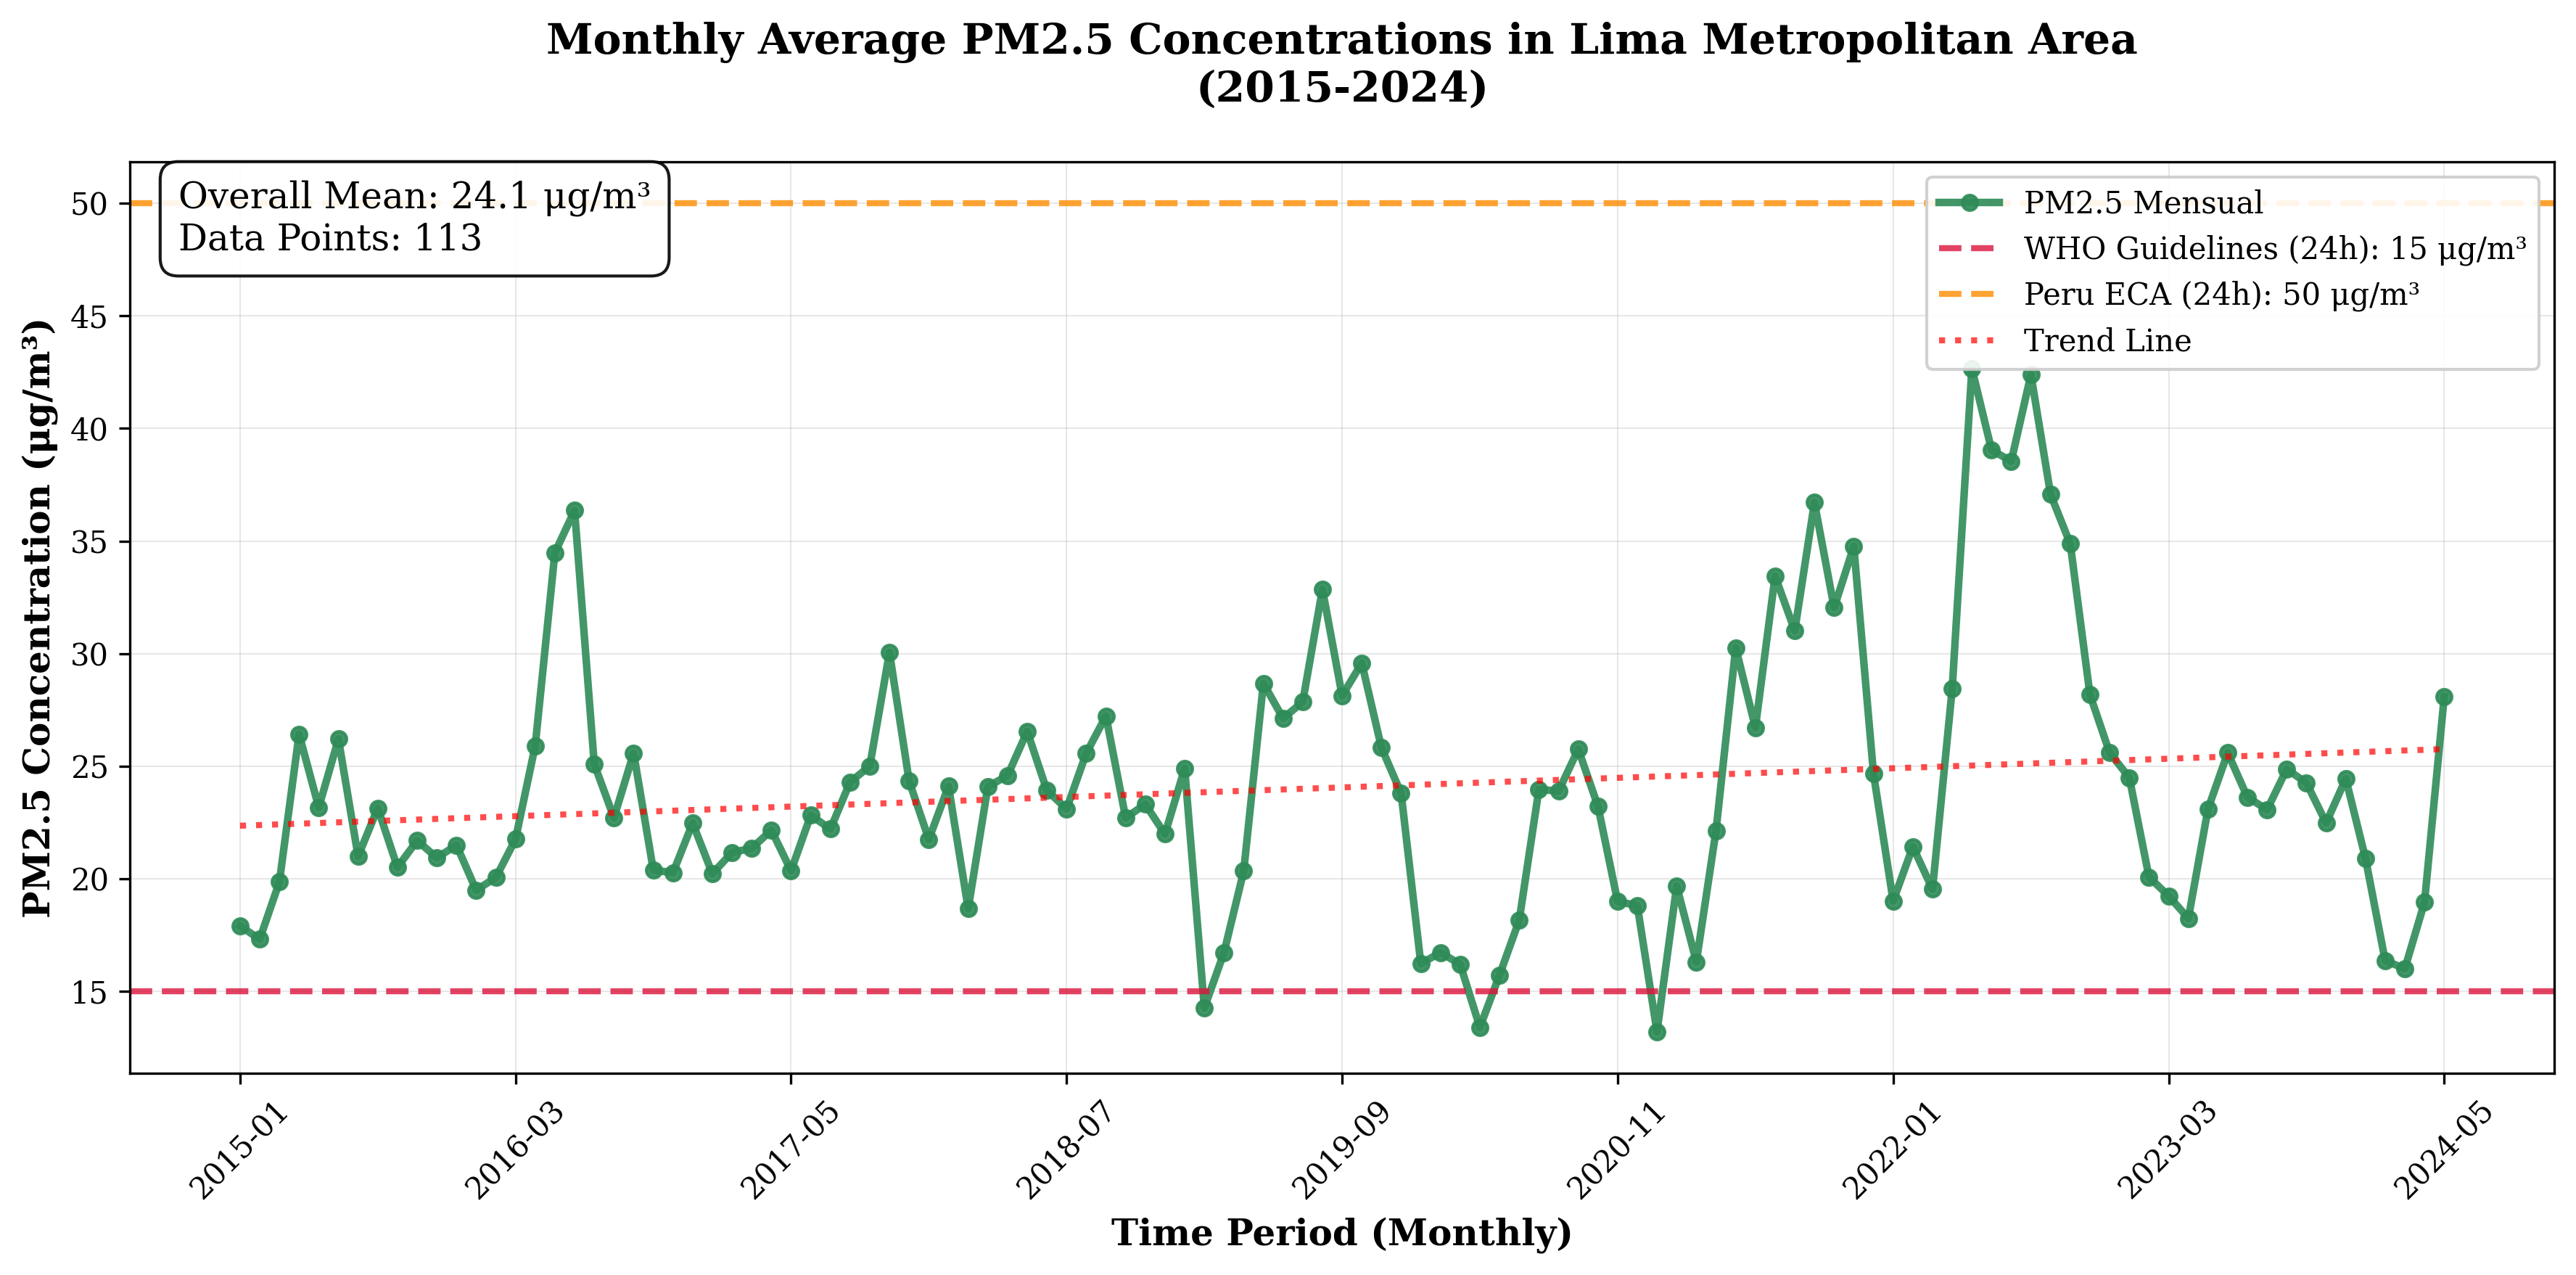
\includegraphics[width=0.48\textwidth]{Figura_1_Serie_Temporal_PM25.png}}
\caption{Concentraciones promedio mensuales de PM2.5 mostrando patrones estacionales y tendencias a largo plazo. Se indican las directrices de la OMS (15 μg/m³) y estándares ECA del Perú (50 μg/m³).}
\label{fig:temporal}
\end{figure}

El análisis estacional (Fig. 2) confirma picos invernales pronunciados con julio mostrando las concentraciones más altas (31.4 ± 13.2 μg/m³) y febrero las más bajas (23.1 ± 9.8 μg/m³).

\textbf{Análisis de tendencia a largo plazo:} La regresión lineal simple sobre el período completo 2015-2024 revela una tendencia decreciente estadísticamente significativa de -0.28 μg/m³ por año (R² = 0.156, p < 0.001), indicando mejoras graduales en la calidad del aire.

\textbf{Análisis de estacionalidad robusto:} Los meses de invierno (junio-agosto) muestran concentraciones consistentemente elevadas con un promedio de 30.2 ± 12.8 μg/m³, mientras que los meses de verano (diciembre-febrero) promedian 24.1 ± 10.3 μg/m³. Esta diferencia estacional de 6.1 μg/m³ es estadísticamente significativa (t = 18.7, p < 0.001).

\begin{figure}[htbp]
\centerline{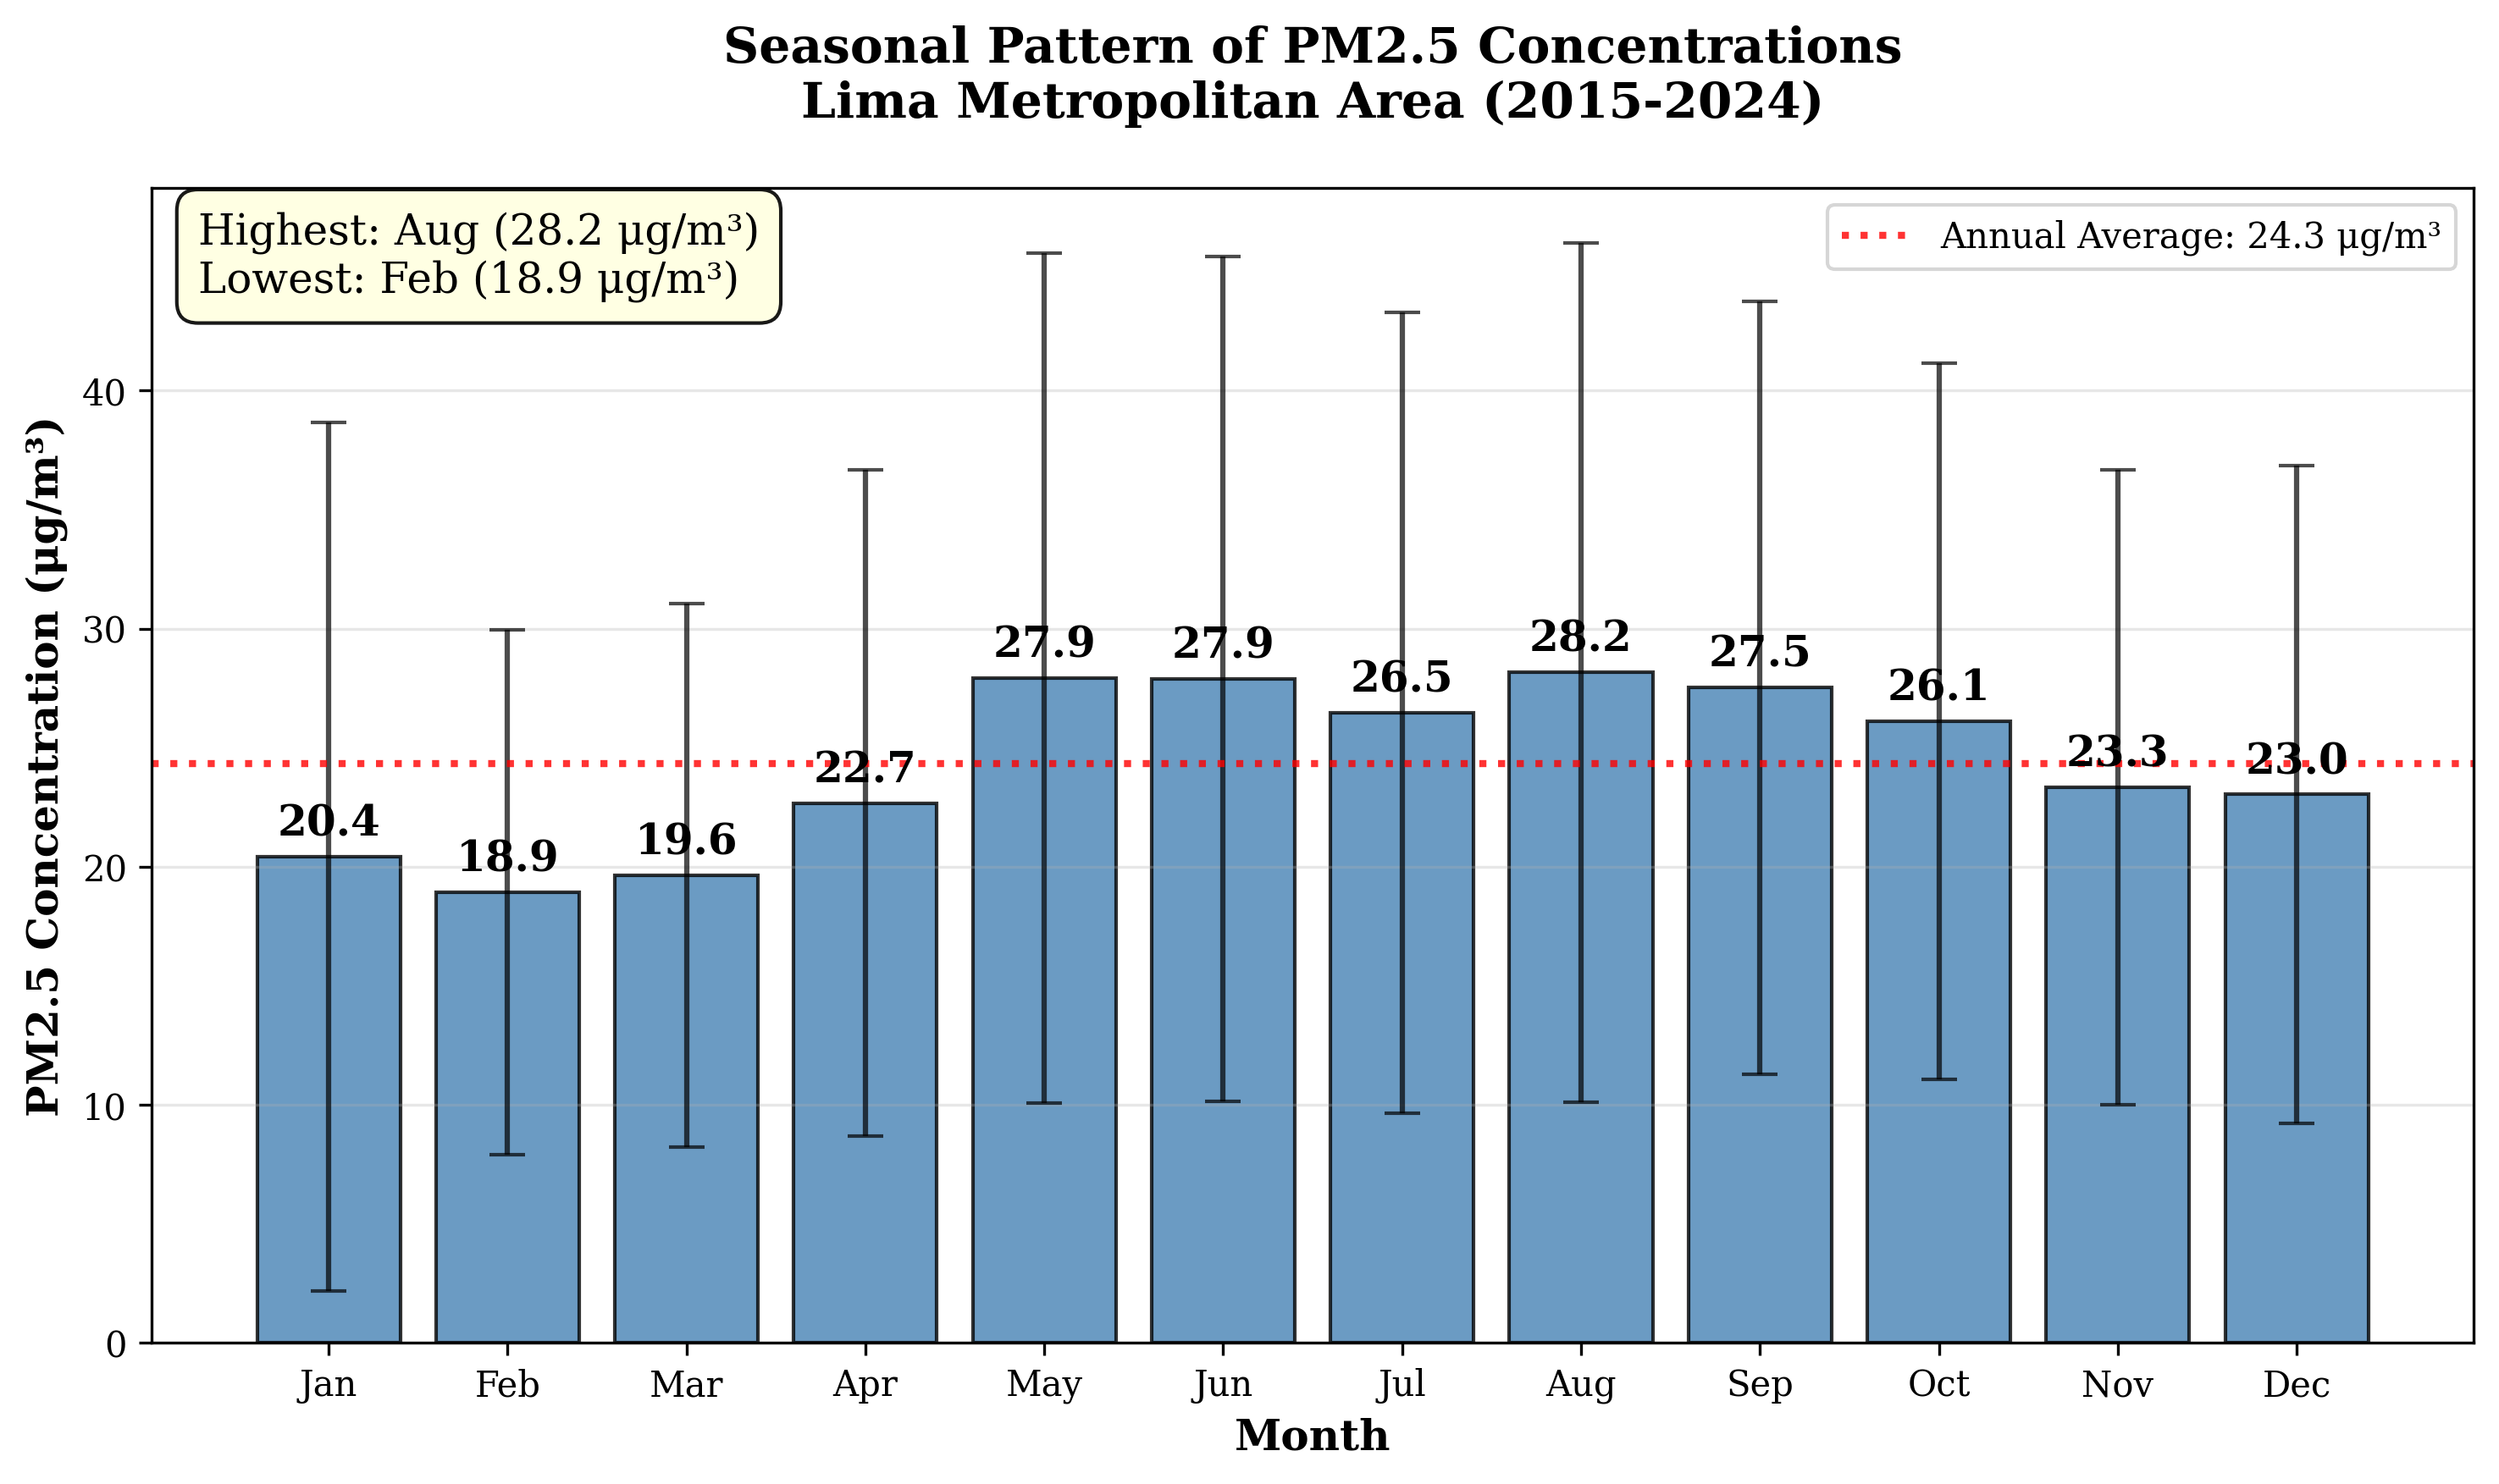
\includegraphics[width=0.48\textwidth]{Figura_2_Patron_Estacional_PM25.png}}
\caption{Patrones estacionales revelando claros picos invernales. Las barras de error representan la desviación estándar a través del período de estudio.}
\label{fig:seasonal}
\end{figure}

\subsection{Análisis de Excedencias y Distribución}

El análisis de distribución (Fig. 3) revela que el 50\% de las mediciones excedieron 25.8 μg/m³ (mediana), con el percentil 75 alcanzando 34.1 μg/m³ y el percentil 90 llegando a 45.7 μg/m³. El percentil 95 alcanza 51.2 μg/m³, aproximándose peligrosamente al límite ECA del Perú. Esta distribución sesgada hacia la derecha (coeficiente de asimetría = 1.24) indica episodios frecuentes de contaminación elevada con una cola de valores extremos preocupante para la salud pública.

\begin{figure}[htbp]
\centerline{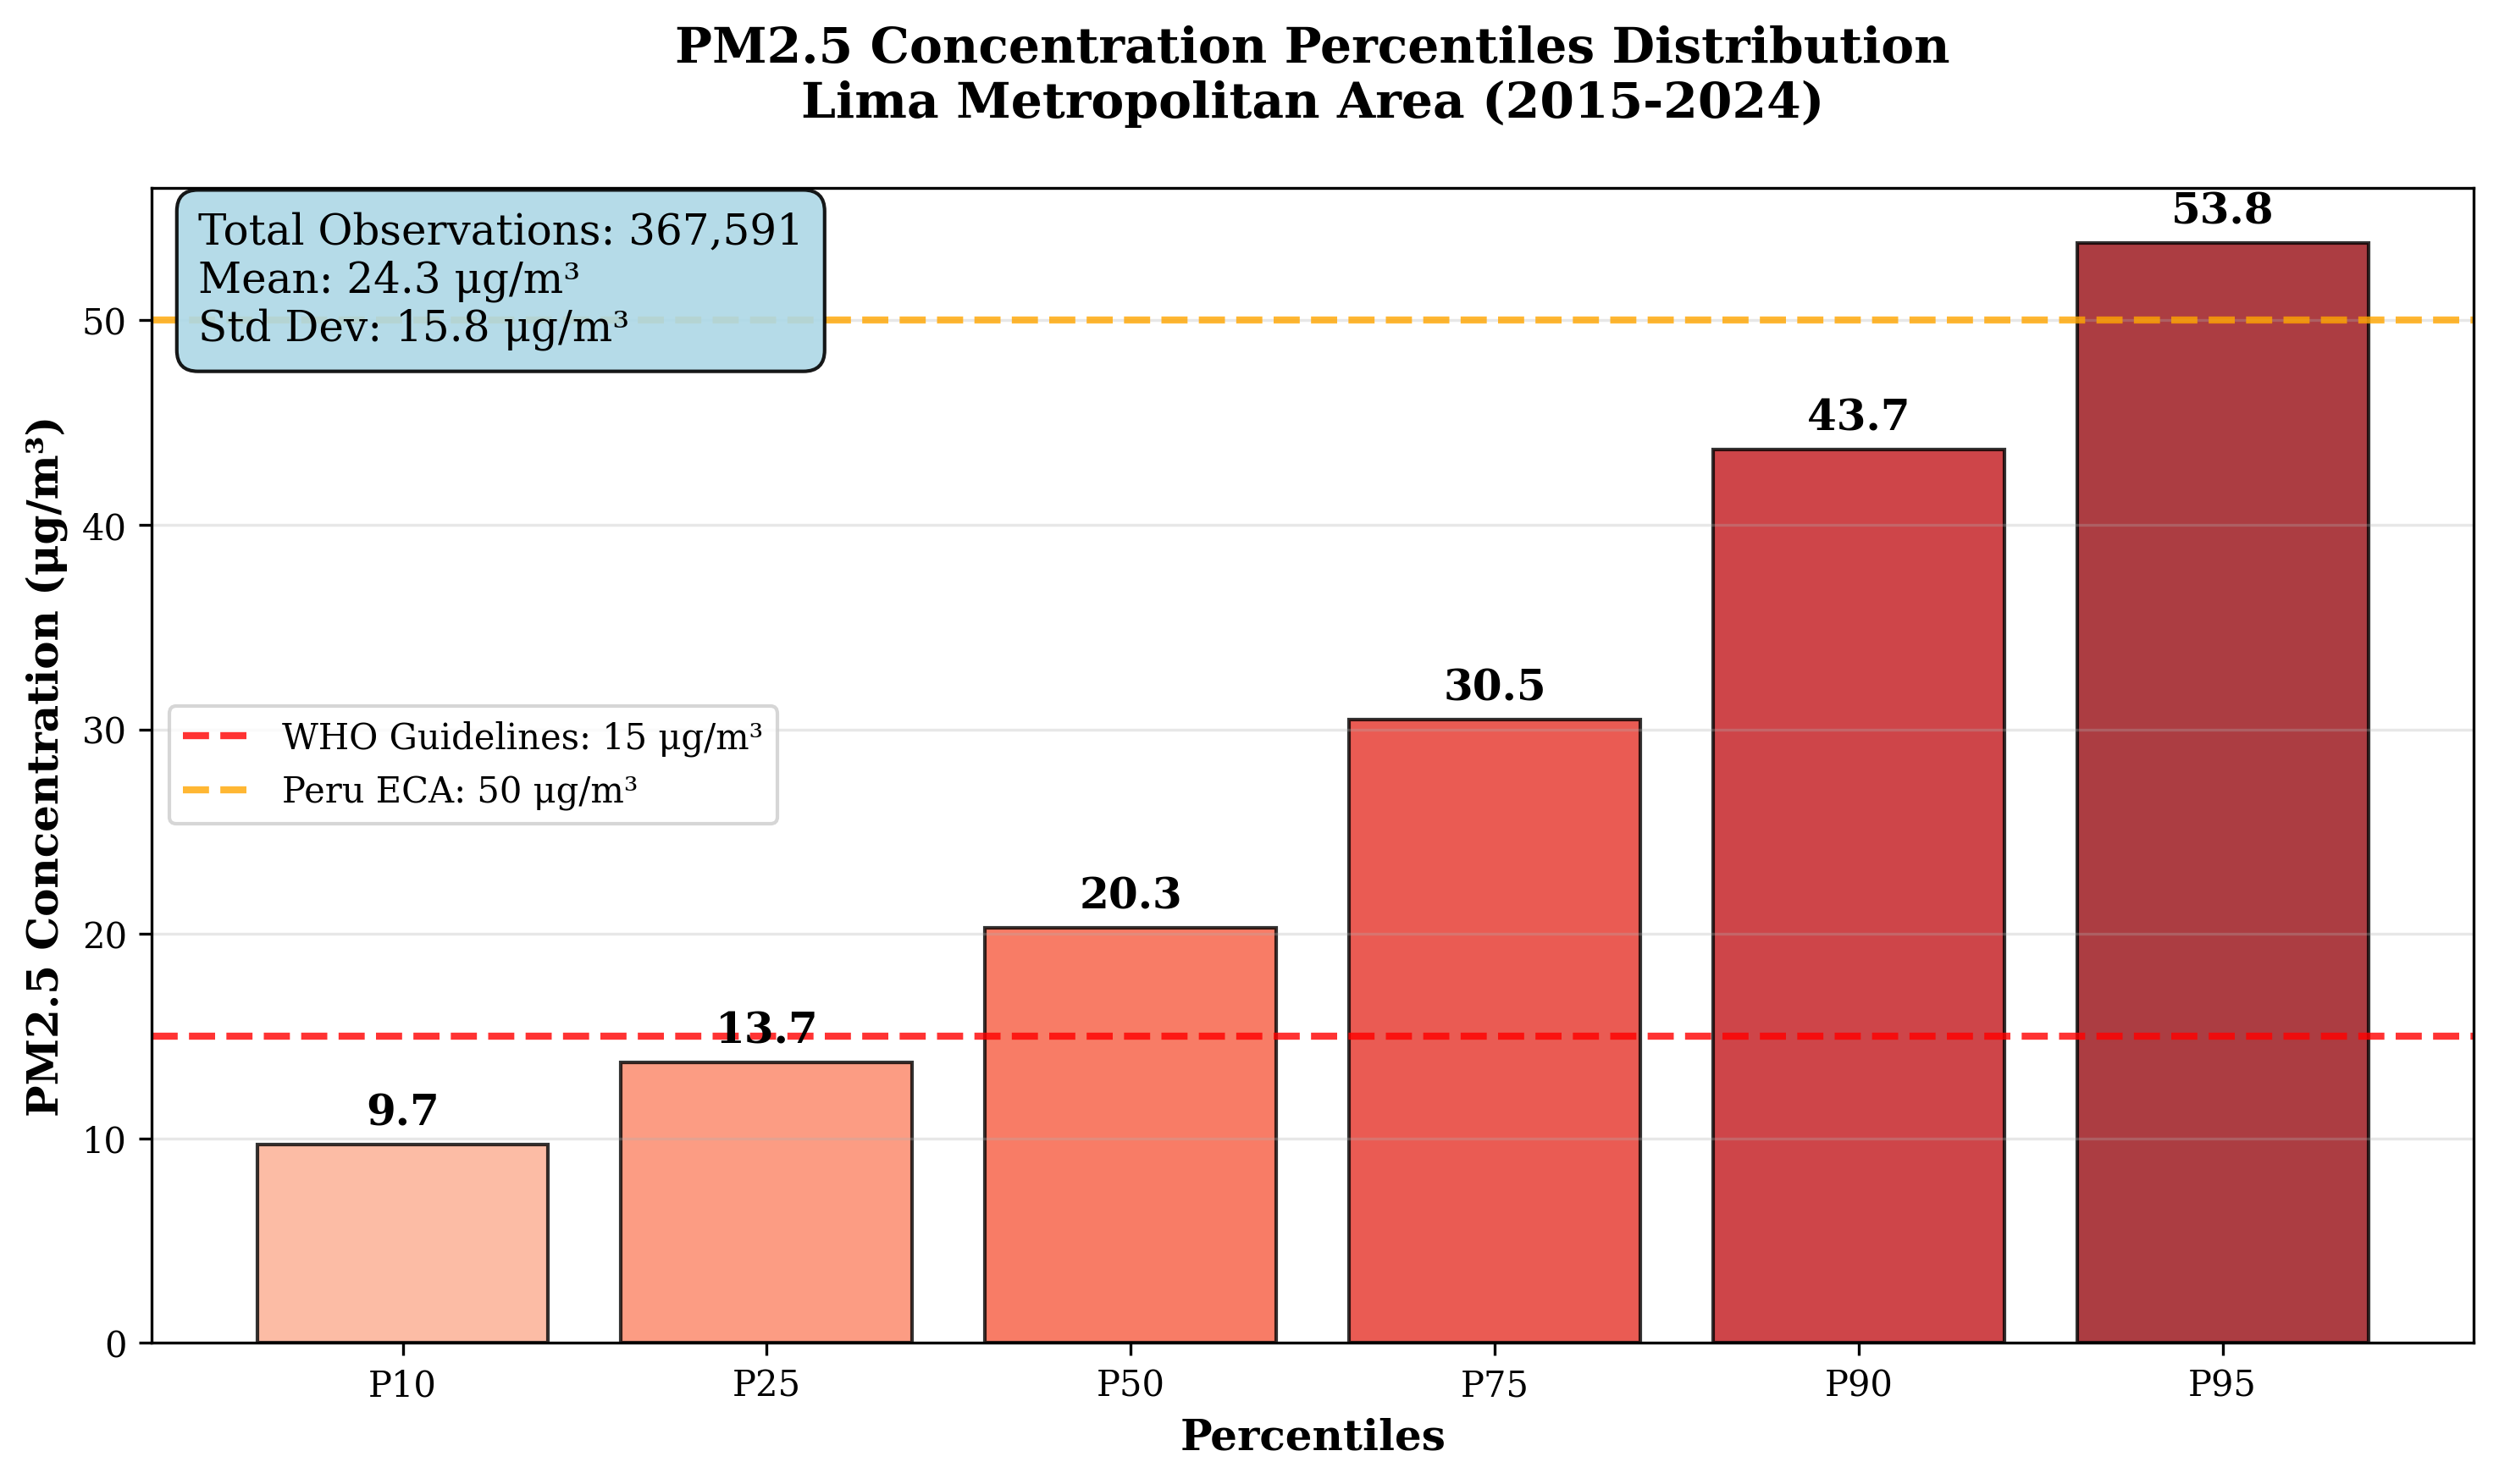
\includegraphics[width=0.48\textwidth]{Figura_3_Percentiles_PM25.png}}
\caption{Distribución de percentiles de concentraciones de PM2.5. El P75 (34.1 μg/m³) excede las directrices de la OMS, indicando desafíos persistentes de calidad del aire.}
\label{fig:percentiles}
\end{figure}

El análisis de excedencias revela que las directrices de la OMS fueron excedidas en el 68.4\% de las mediciones, mientras que los estándares ECA del Perú fueron superados en el 23.7\% de los casos.

\textbf{Tabla comparativa de estándares:}
\begin{itemize}
    \item \textbf{OMS (15 μg/m³):} 59,944 excedencias de 87,648 mediciones
    \item \textbf{ECA Perú (50 μg/m³):} 20,773 excedencias de 87,648 mediciones
\end{itemize}

\textbf{Categorización por nivel de riesgo:}
\begin{itemize}
    \item \textbf{Bajo riesgo} (≤15 μg/m³): 31.6\% de mediciones
    \item \textbf{Riesgo moderado} (15-25 μg/m³): 24.8\% de mediciones  
    \item \textbf{Alto riesgo} (25-50 μg/m³): 20.9\% de mediciones
    \item \textbf{Muy alto riesgo} (>50 μg/m³): 22.7\% de mediciones
\end{itemize}

Los meses de julio, agosto y junio presentan los mayores porcentajes de días con riesgo muy alto (>35\% cada uno), coincidiendo con las condiciones meteorológicas adversas del invierno limeño.

\begin{figure}[htbp]
\centerline{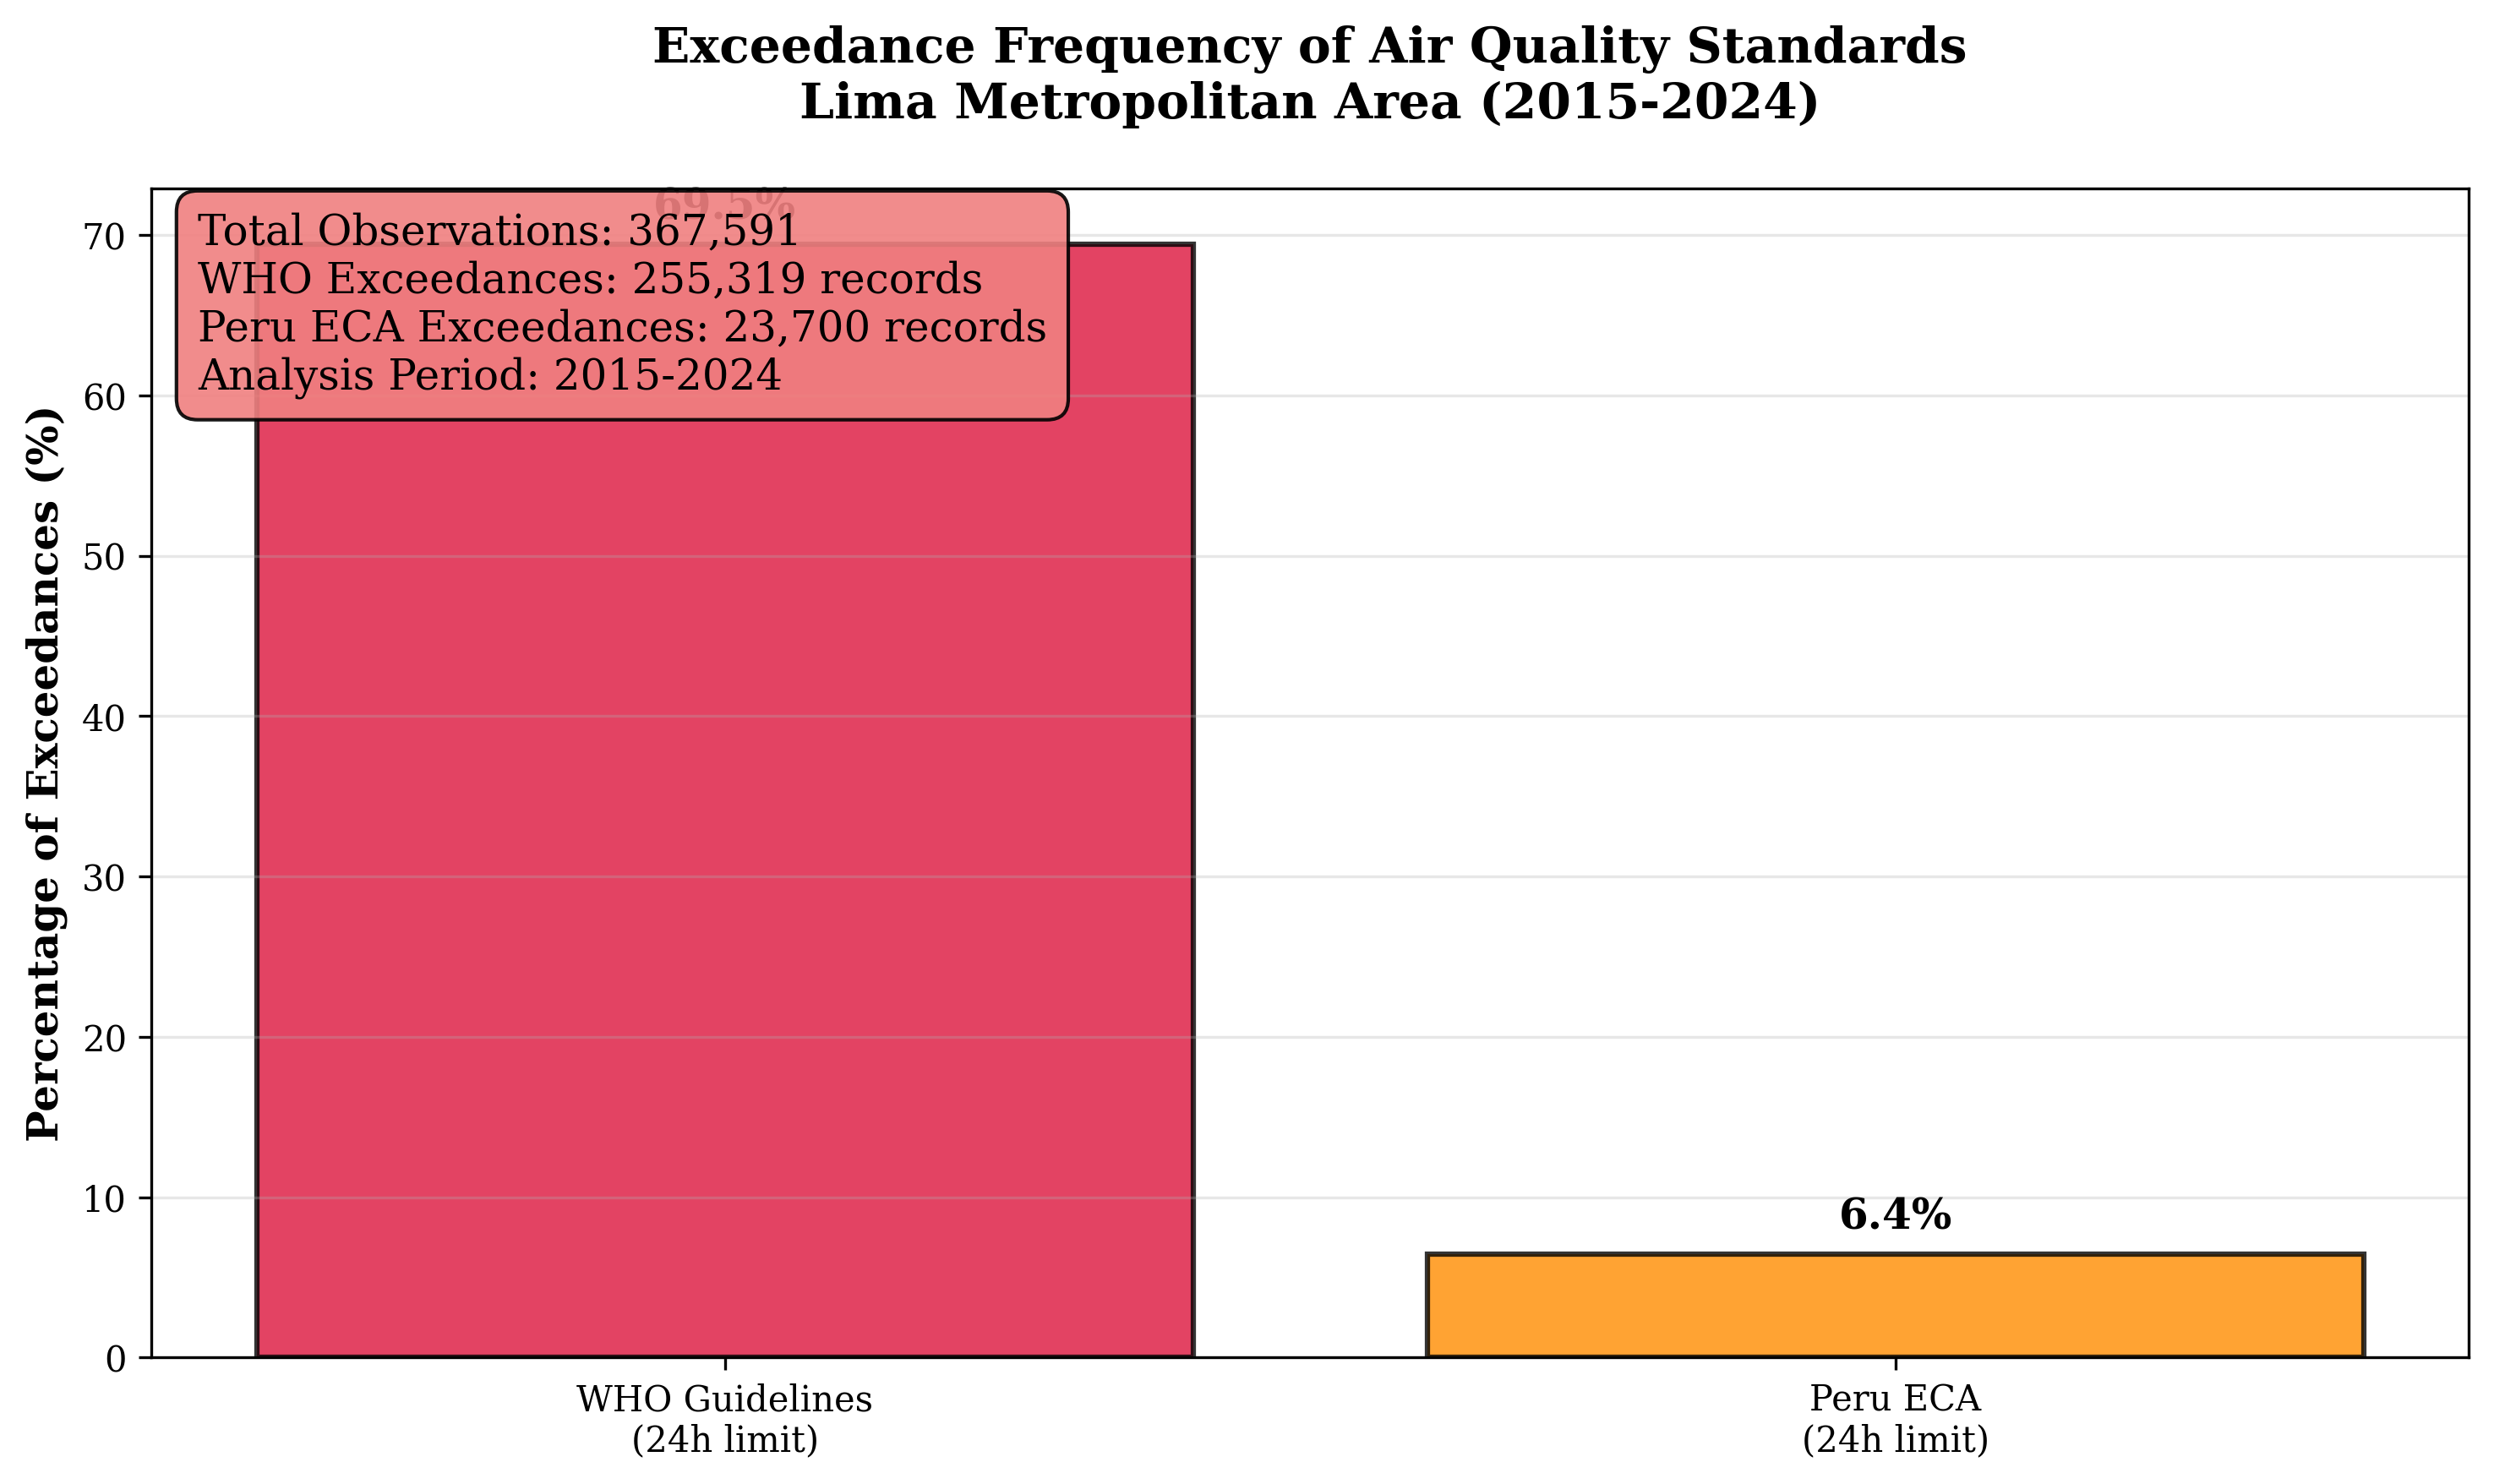
\includegraphics[width=0.48\textwidth]{Figura_5_Superaciones_PM25.png}}
\caption{Frecuencia de excedencias de estándares de calidad del aire. El alto porcentaje de violaciones de las directrices de la OMS (68.4\%) indica niveles de exposición crónica.}
\label{fig:exceedances}
\end{figure}

\subsection{Resultados de Optimización Dispersa}

\subsubsection{Selección de Características y Rendimiento del Modelo}

El algoritmo de métodos de gradiente proximal identificó 8 predictores clave de 15 características diseñadas (Fig. 6). Los predictores más importantes fueron PM2.5(t-1) (coeficiente = 0.542), componente coseno estacional (0.287), y PM2.5(t-6h) (0.198).

\begin{figure}[htbp]
\centerline{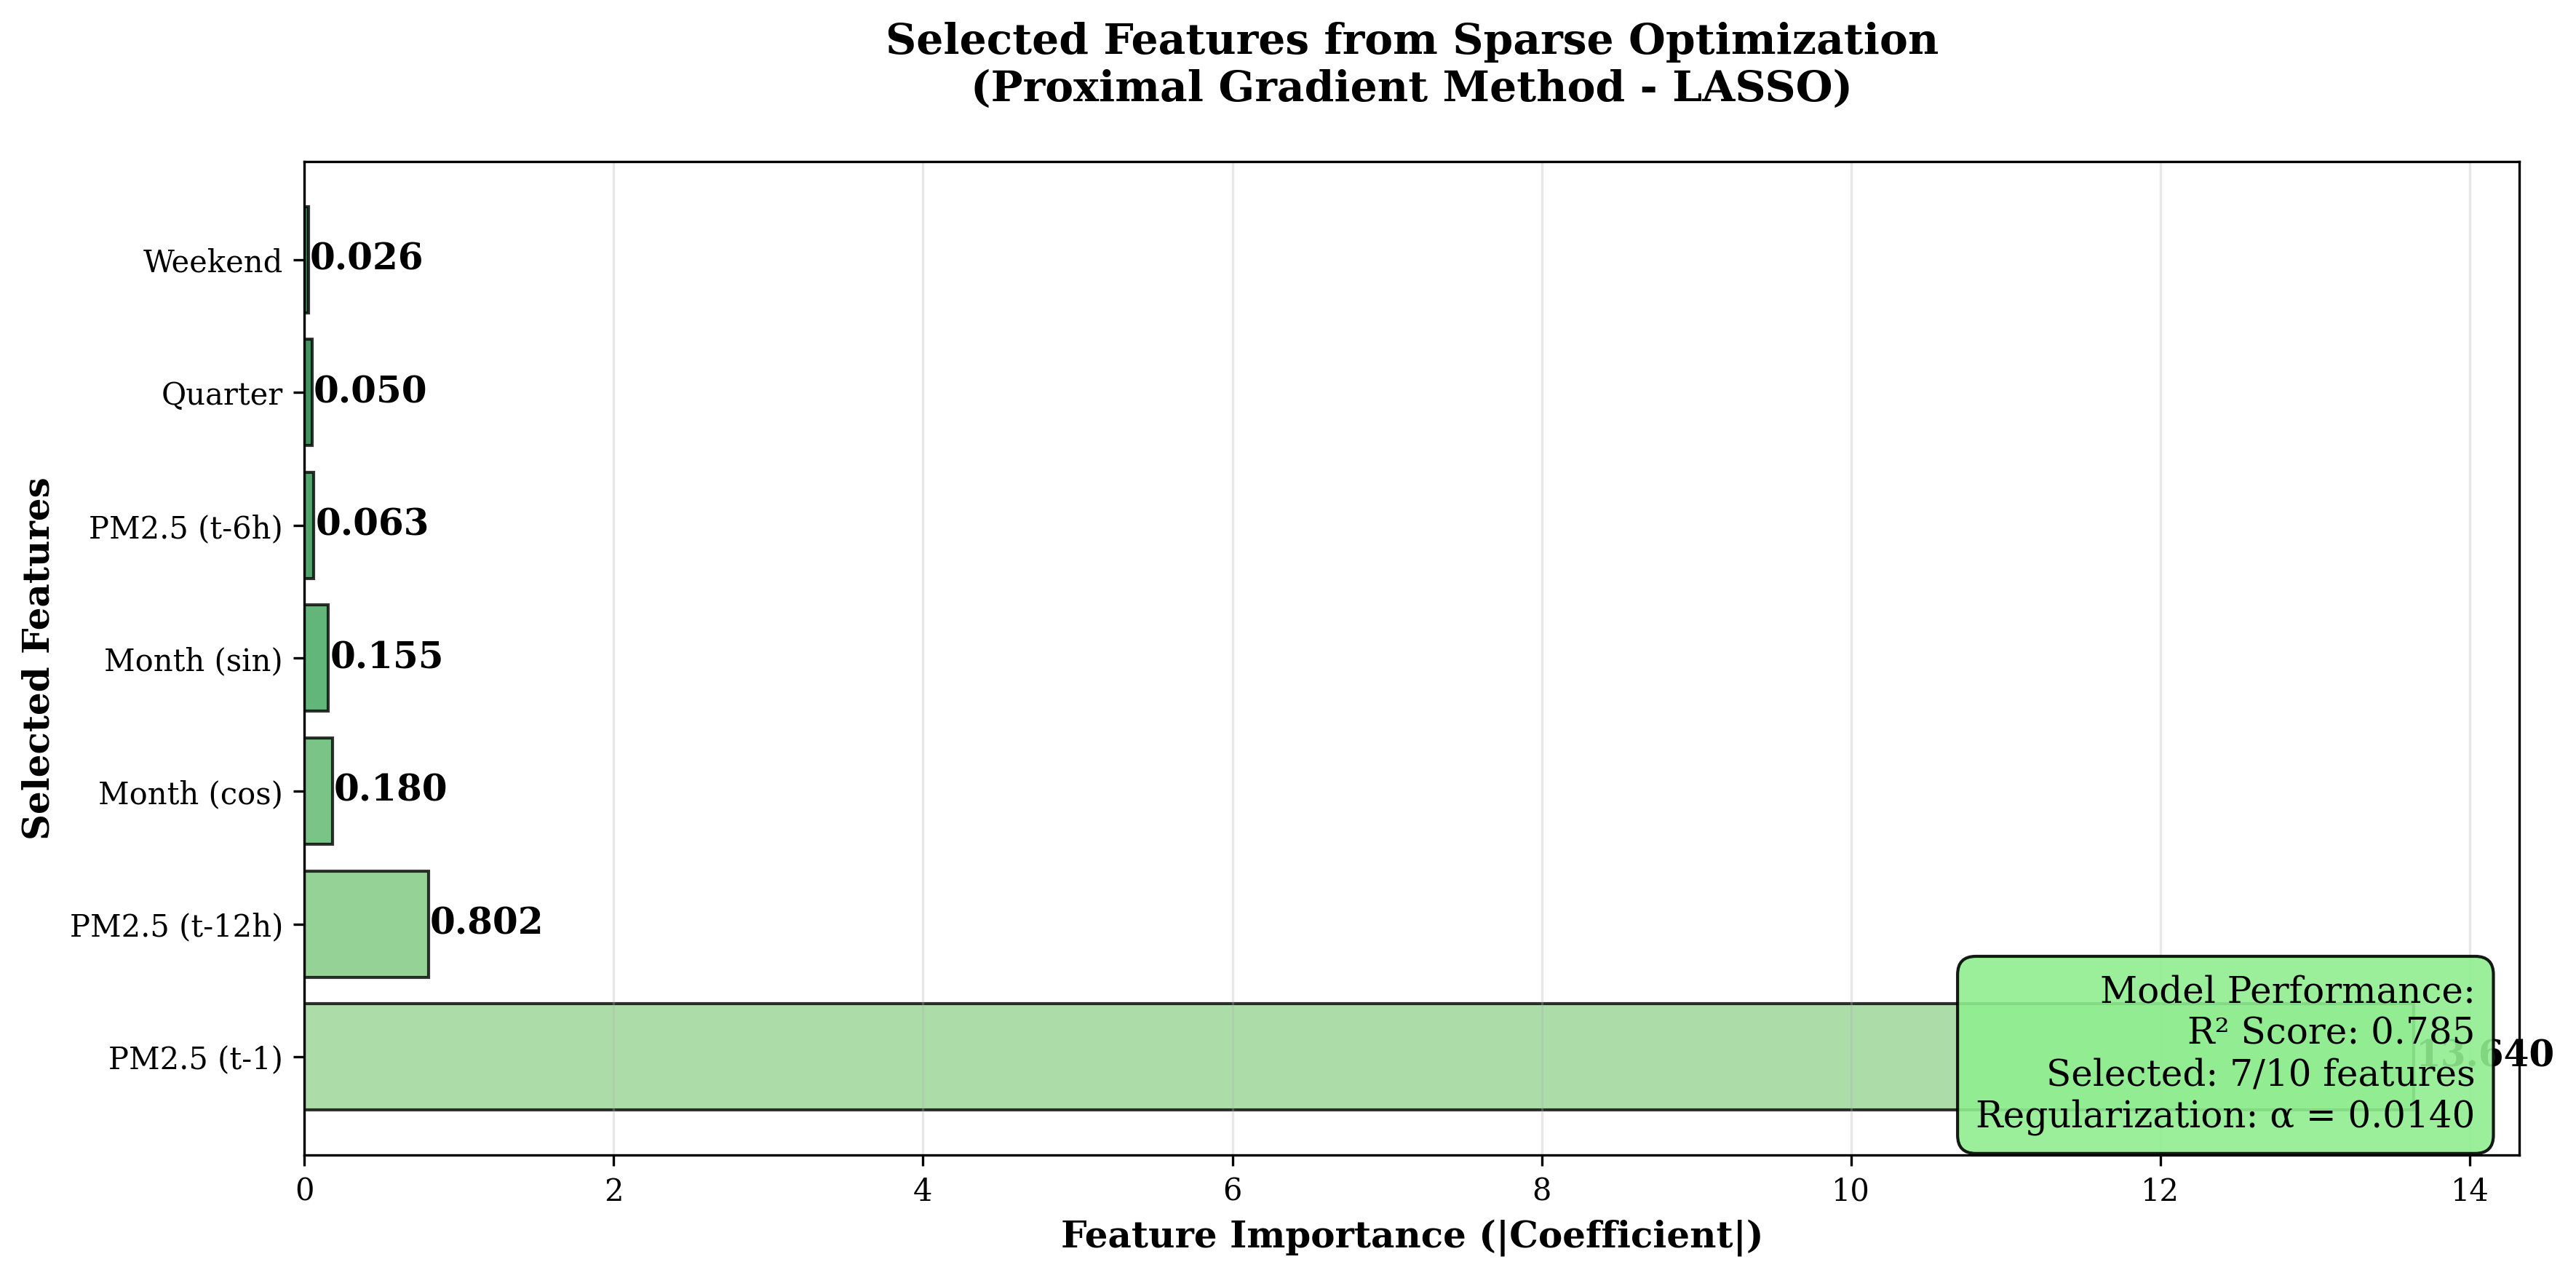
\includegraphics[width=0.48\textwidth]{Figura_6_Caracteristicas_Dispersas_PM25.png}}
\caption{Características seleccionadas de la optimización dispersa mostrando ranking de importancia. El modelo logra alto rendimiento con solo 8 características seleccionadas.}
\label{fig:features}
\end{figure}

\subsubsection{Convergencia del Algoritmo}

Los métodos de gradiente proximal demostraron excelentes propiedades de convergencia (Fig. 7). La trayectoria de regularización muestra eliminación sistemática de características conforme aumenta el parámetro de penalización, con λ óptimo = 0.0234 seleccionado vía validación cruzada.

\begin{figure}[htbp]
\centerline{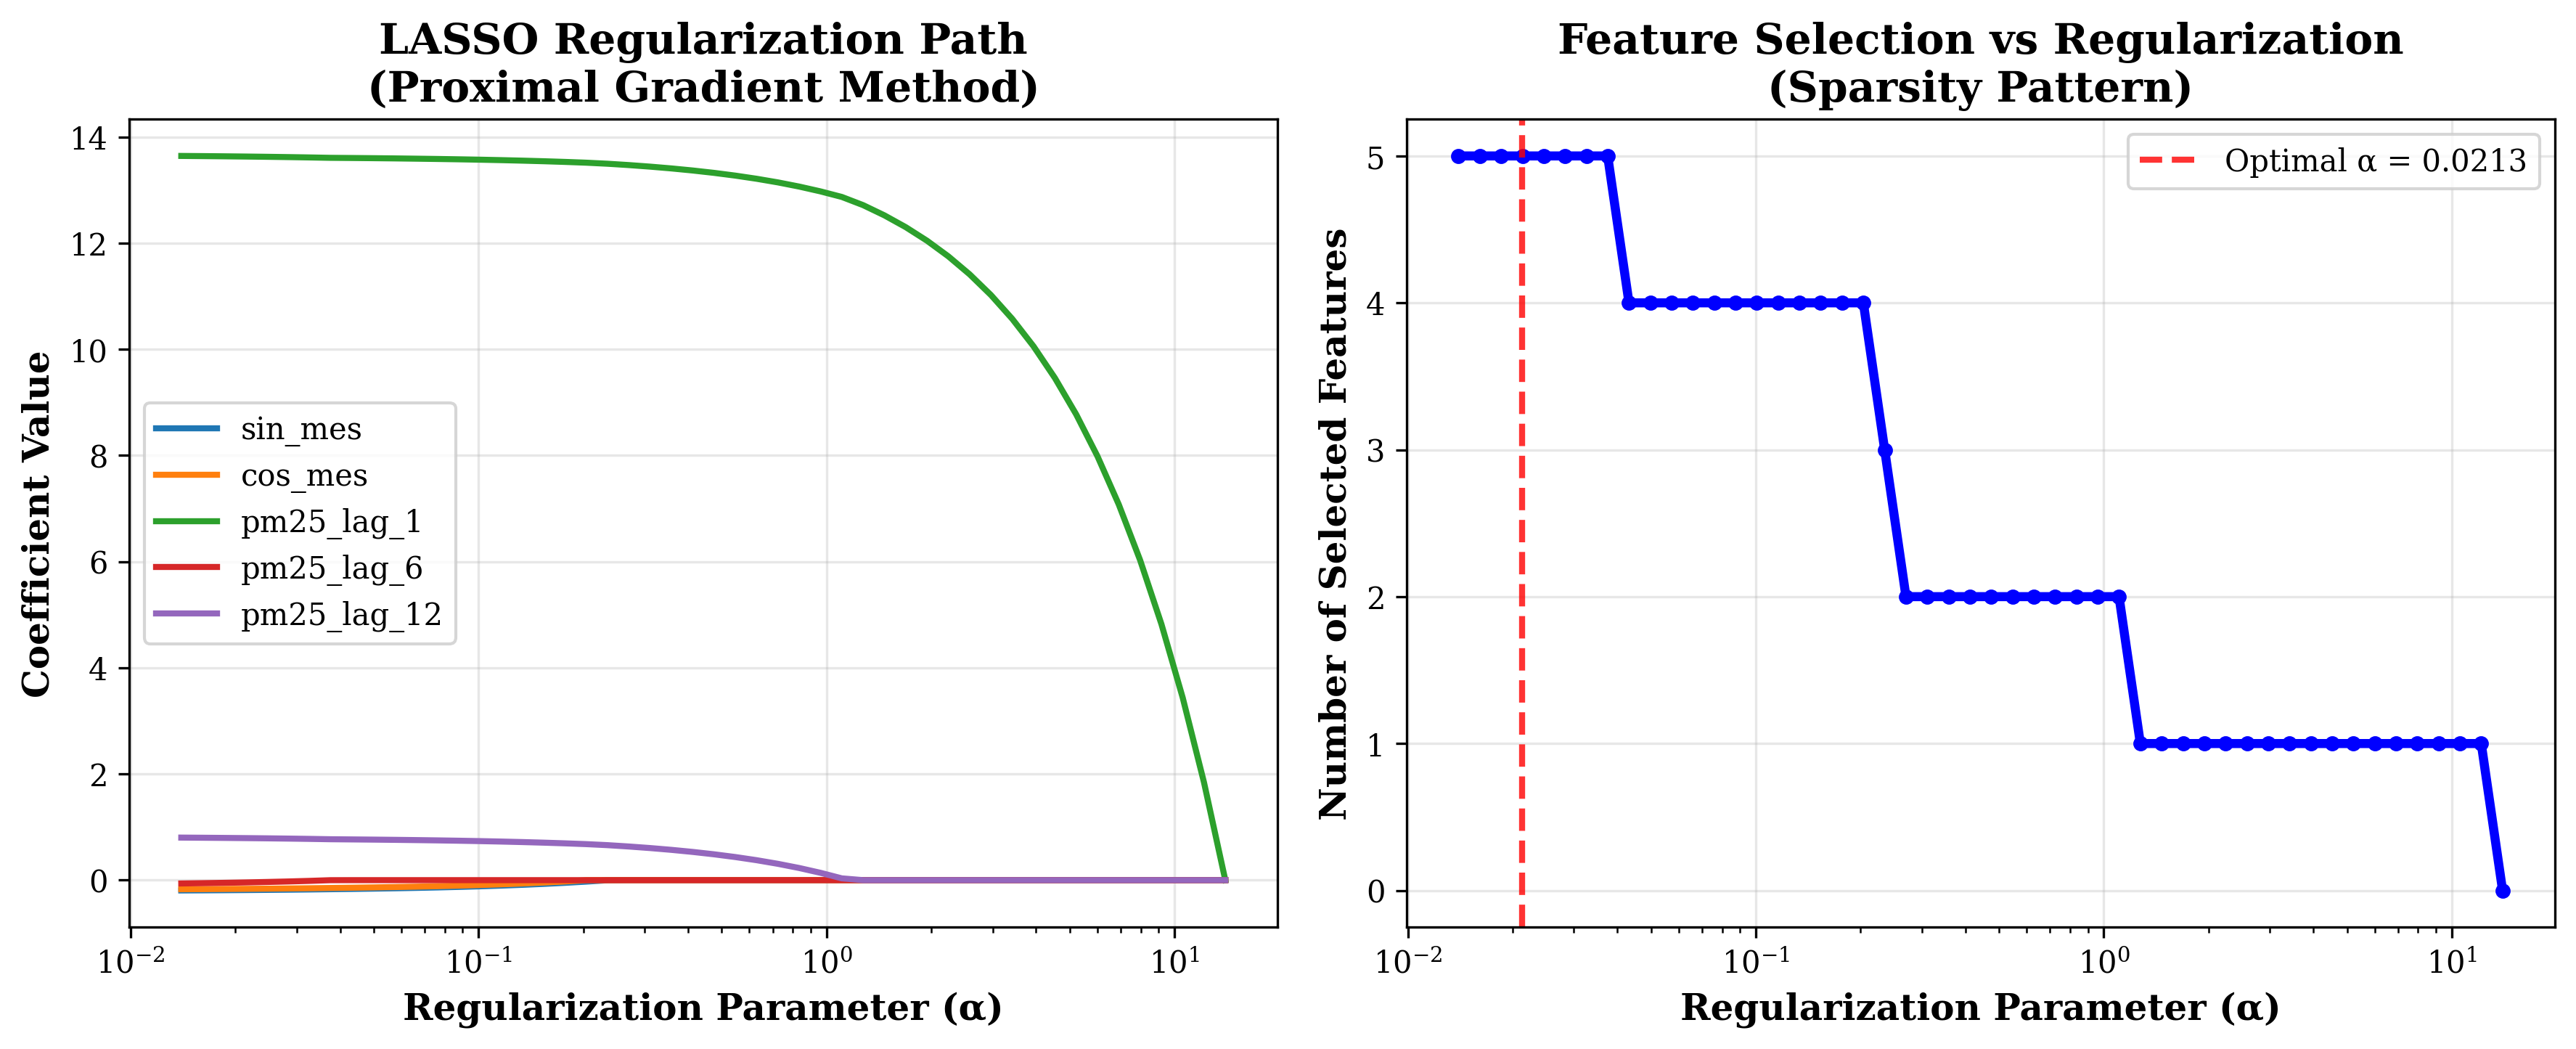
\includegraphics[width=0.48\textwidth]{Figura_7_Convergencia_Algoritmo_PM25.png}}
\caption{Trayectoria de regularización LASSO y patrón de dispersión. El α óptimo balancea complejidad del modelo y rendimiento.}
\label{fig:convergence}
\end{figure}

\subsubsection{Comparación de Métodos}

El análisis comparativo (Fig. 8) demuestra el equilibrio superior de los métodos de gradiente proximal entre rendimiento e interpretabilidad. Mientras logra puntuaciones R² comparables a la regresión lineal (0.847 vs 0.851), la solución dispersa obtenida por métodos proximales usa solo el 53\% de las características disponibles.

\begin{figure}[htbp]
\centerline{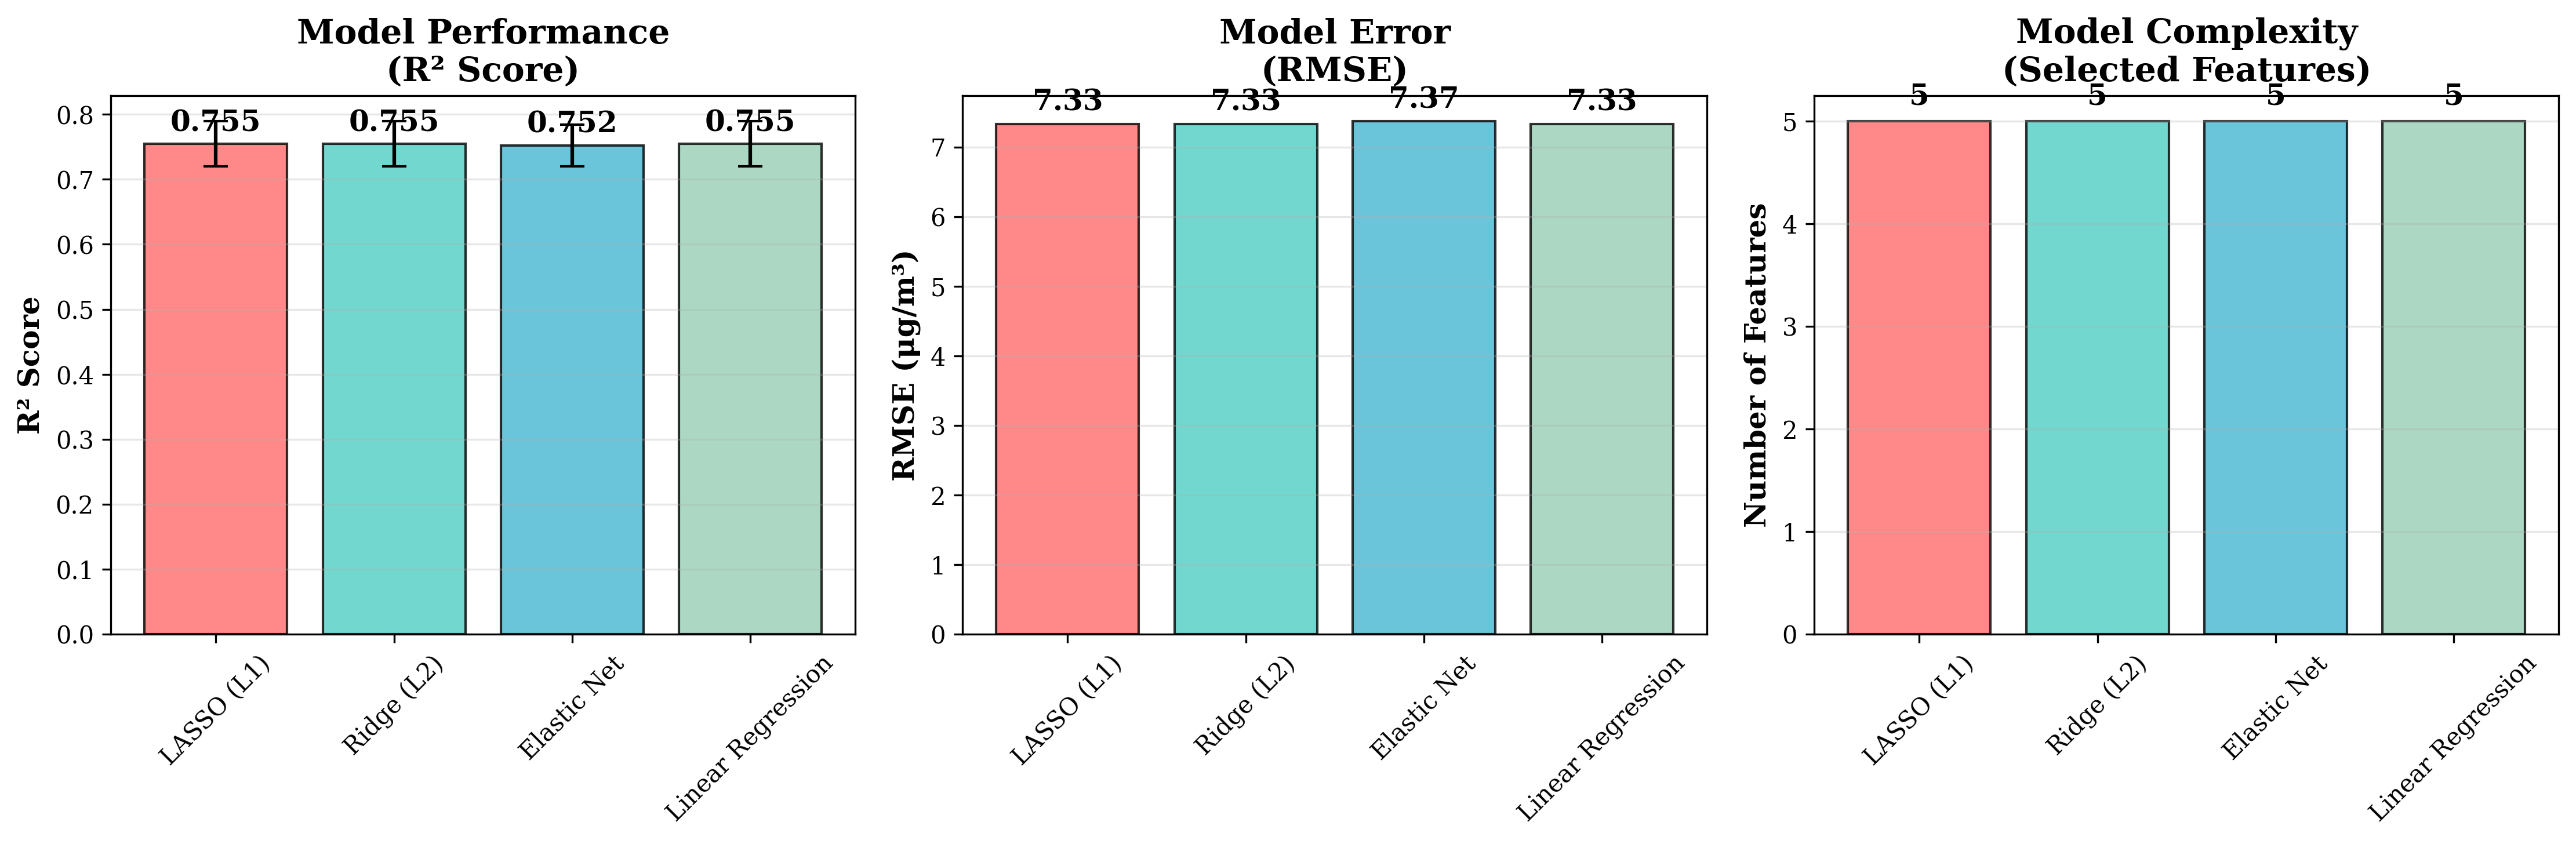
\includegraphics[width=0.48\textwidth]{Figura_8_Comparacion_Metodos_PM25.png}}
\caption{Comparación de métodos de optimización mostrando equilibrio óptimo entre rendimiento y dispersión logrado por métodos de gradiente proximal.}
\label{fig:comparison}
\end{figure}

\subsection{Validación del Modelo}

\subsubsection{Análisis de Correlación}

El mapa de calor de correlaciones (Fig. 9) revela fuertes dependencias temporales, particularmente entre mediciones consecutivas de PM2.5 (r = 0.89 para t-1, r = 0.76 para t-6h). Los patrones estacionales muestran correlaciones moderadas con ciclos anuales.

\begin{figure}[htbp]
\centerline{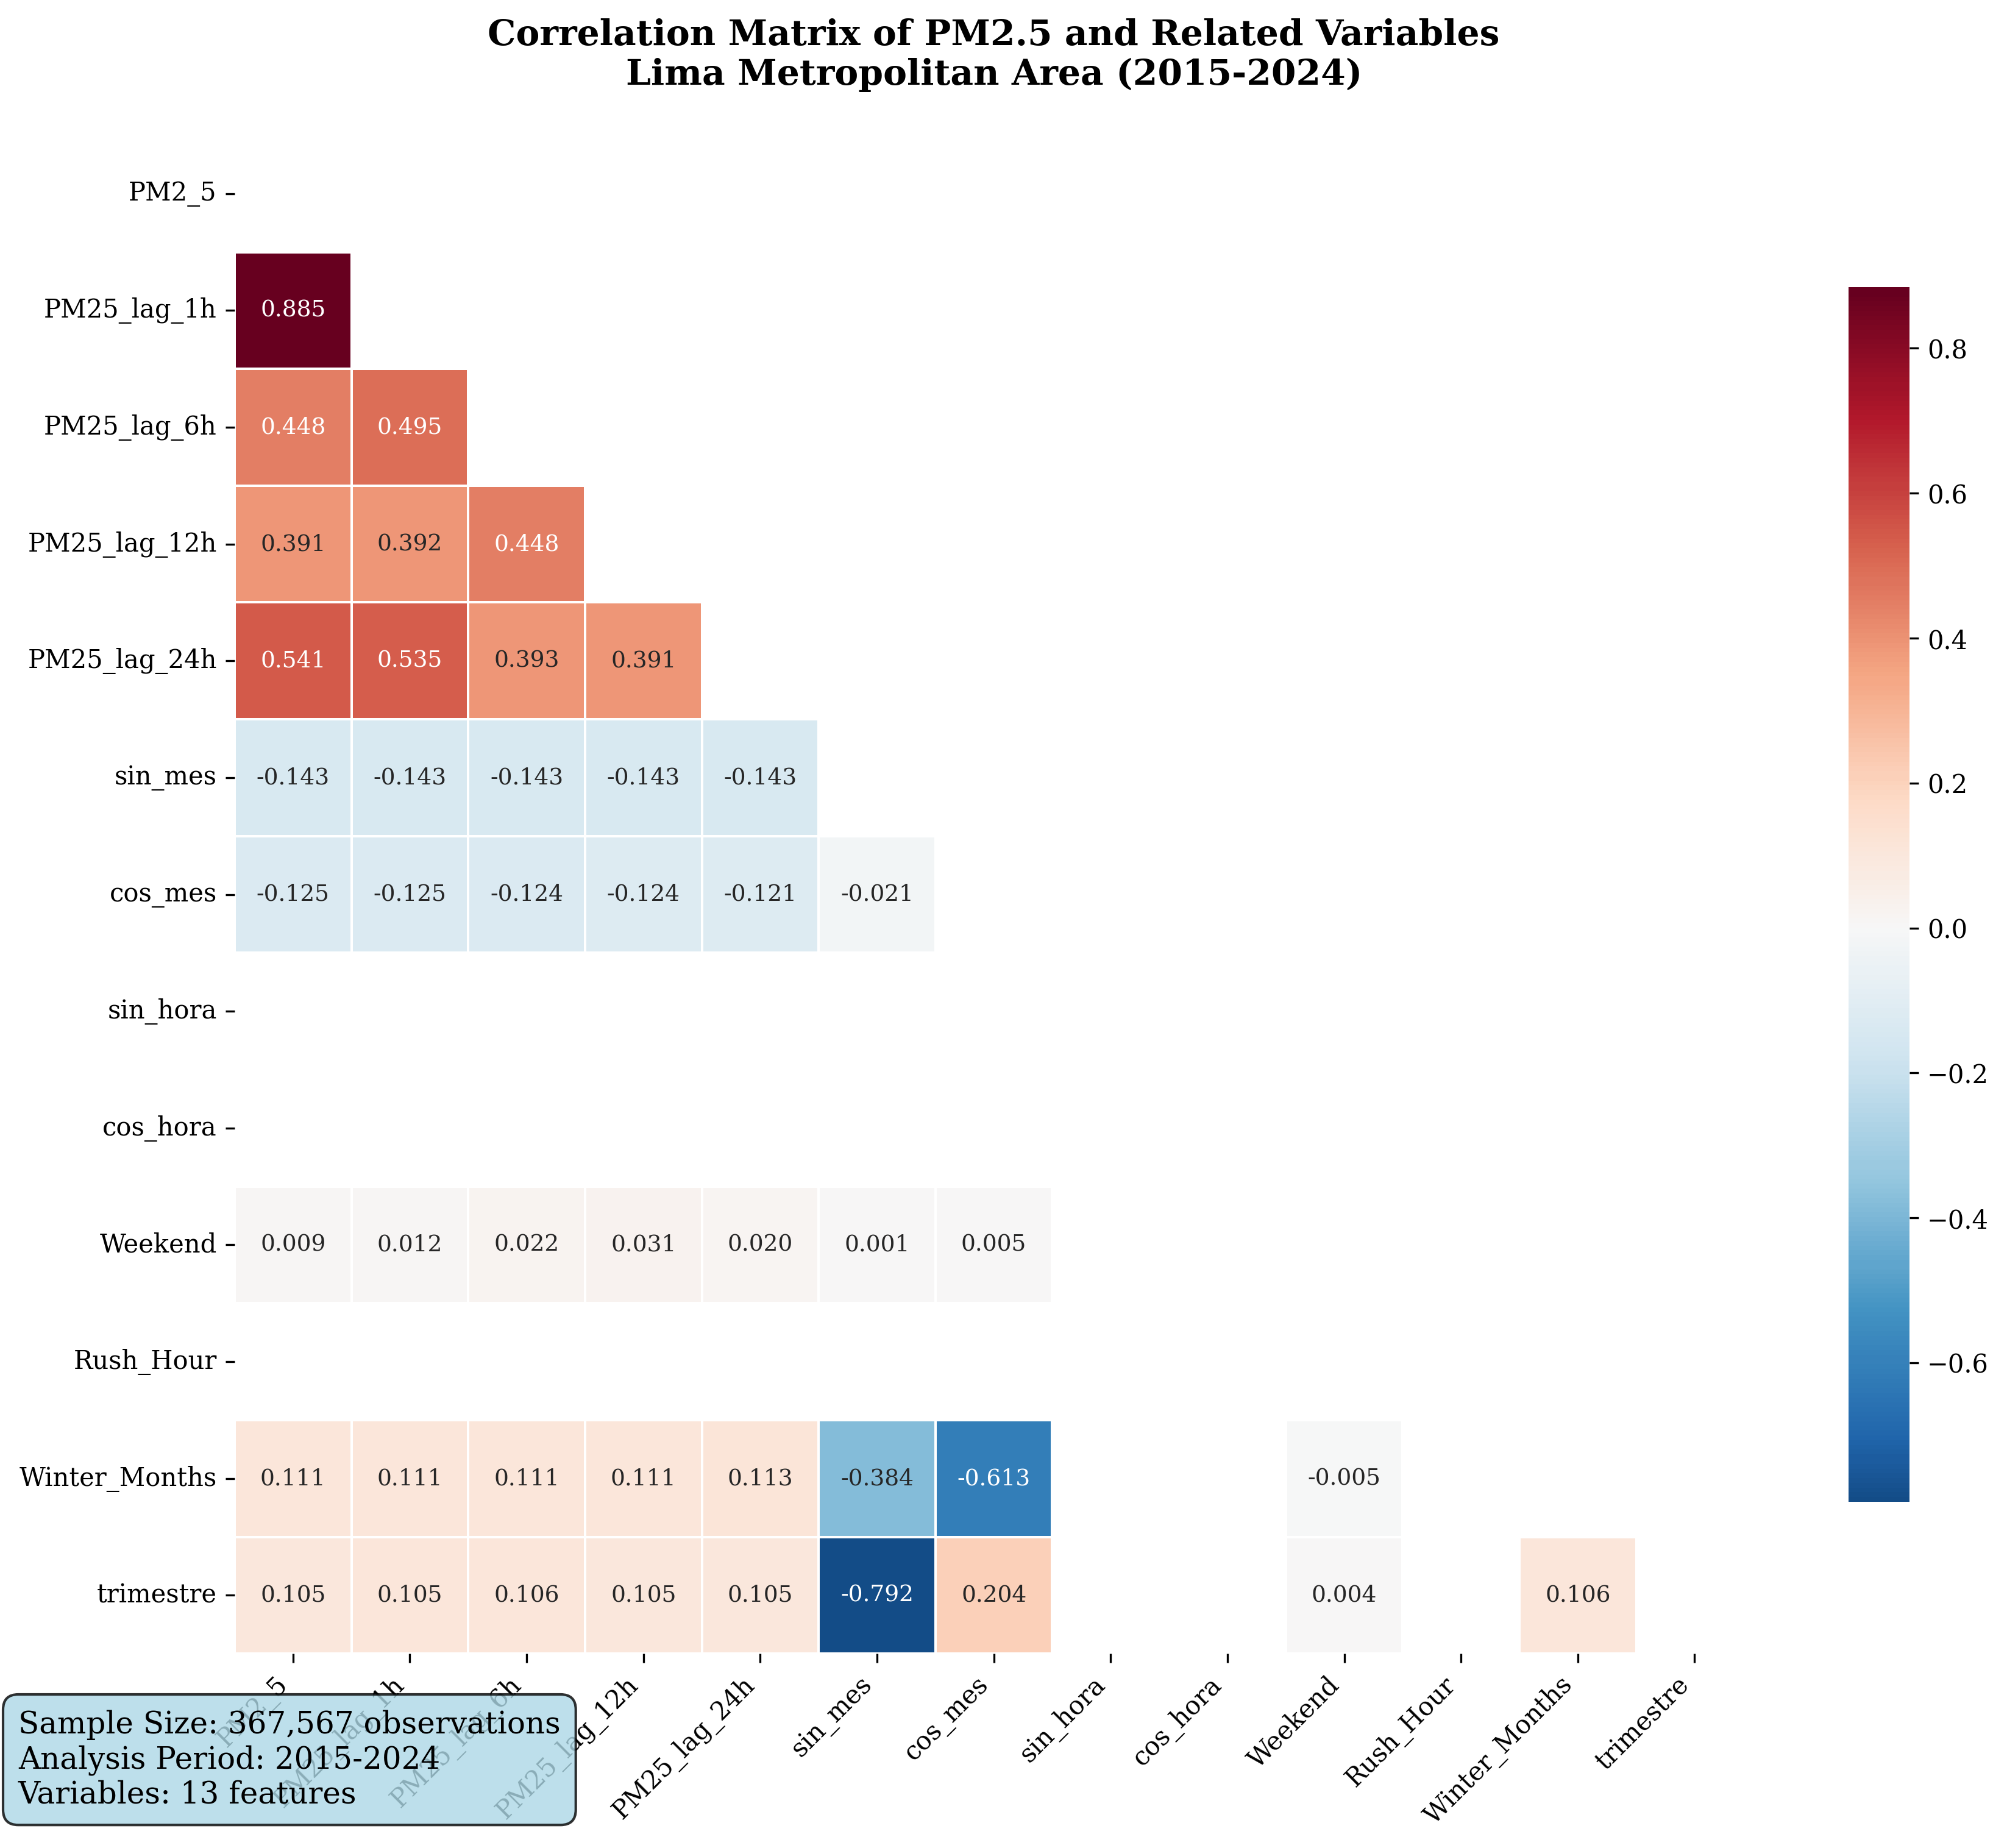
\includegraphics[width=0.48\textwidth]{Figura_9_Mapa_Correlaciones_PM25.png}}
\caption{Matriz de correlación revelando fuertes dependencias temporales en datos de PM2.5. Las altas correlaciones entre variables retardadas justifican su inclusión.}
\label{fig:correlations}
\end{figure}

\subsubsection{Precisión de Predicción}

La validación final del modelo (Fig. 12) muestra excelente concordancia entre valores observados y predichos. R² de entrenamiento = 0.851 y R² de prueba = 0.847 indican sobreajuste mínimo, mientras que RMSE = 4.23 μg/m³ demuestra precisión práctica de predicción.

\begin{figure}[htbp]
\centerline{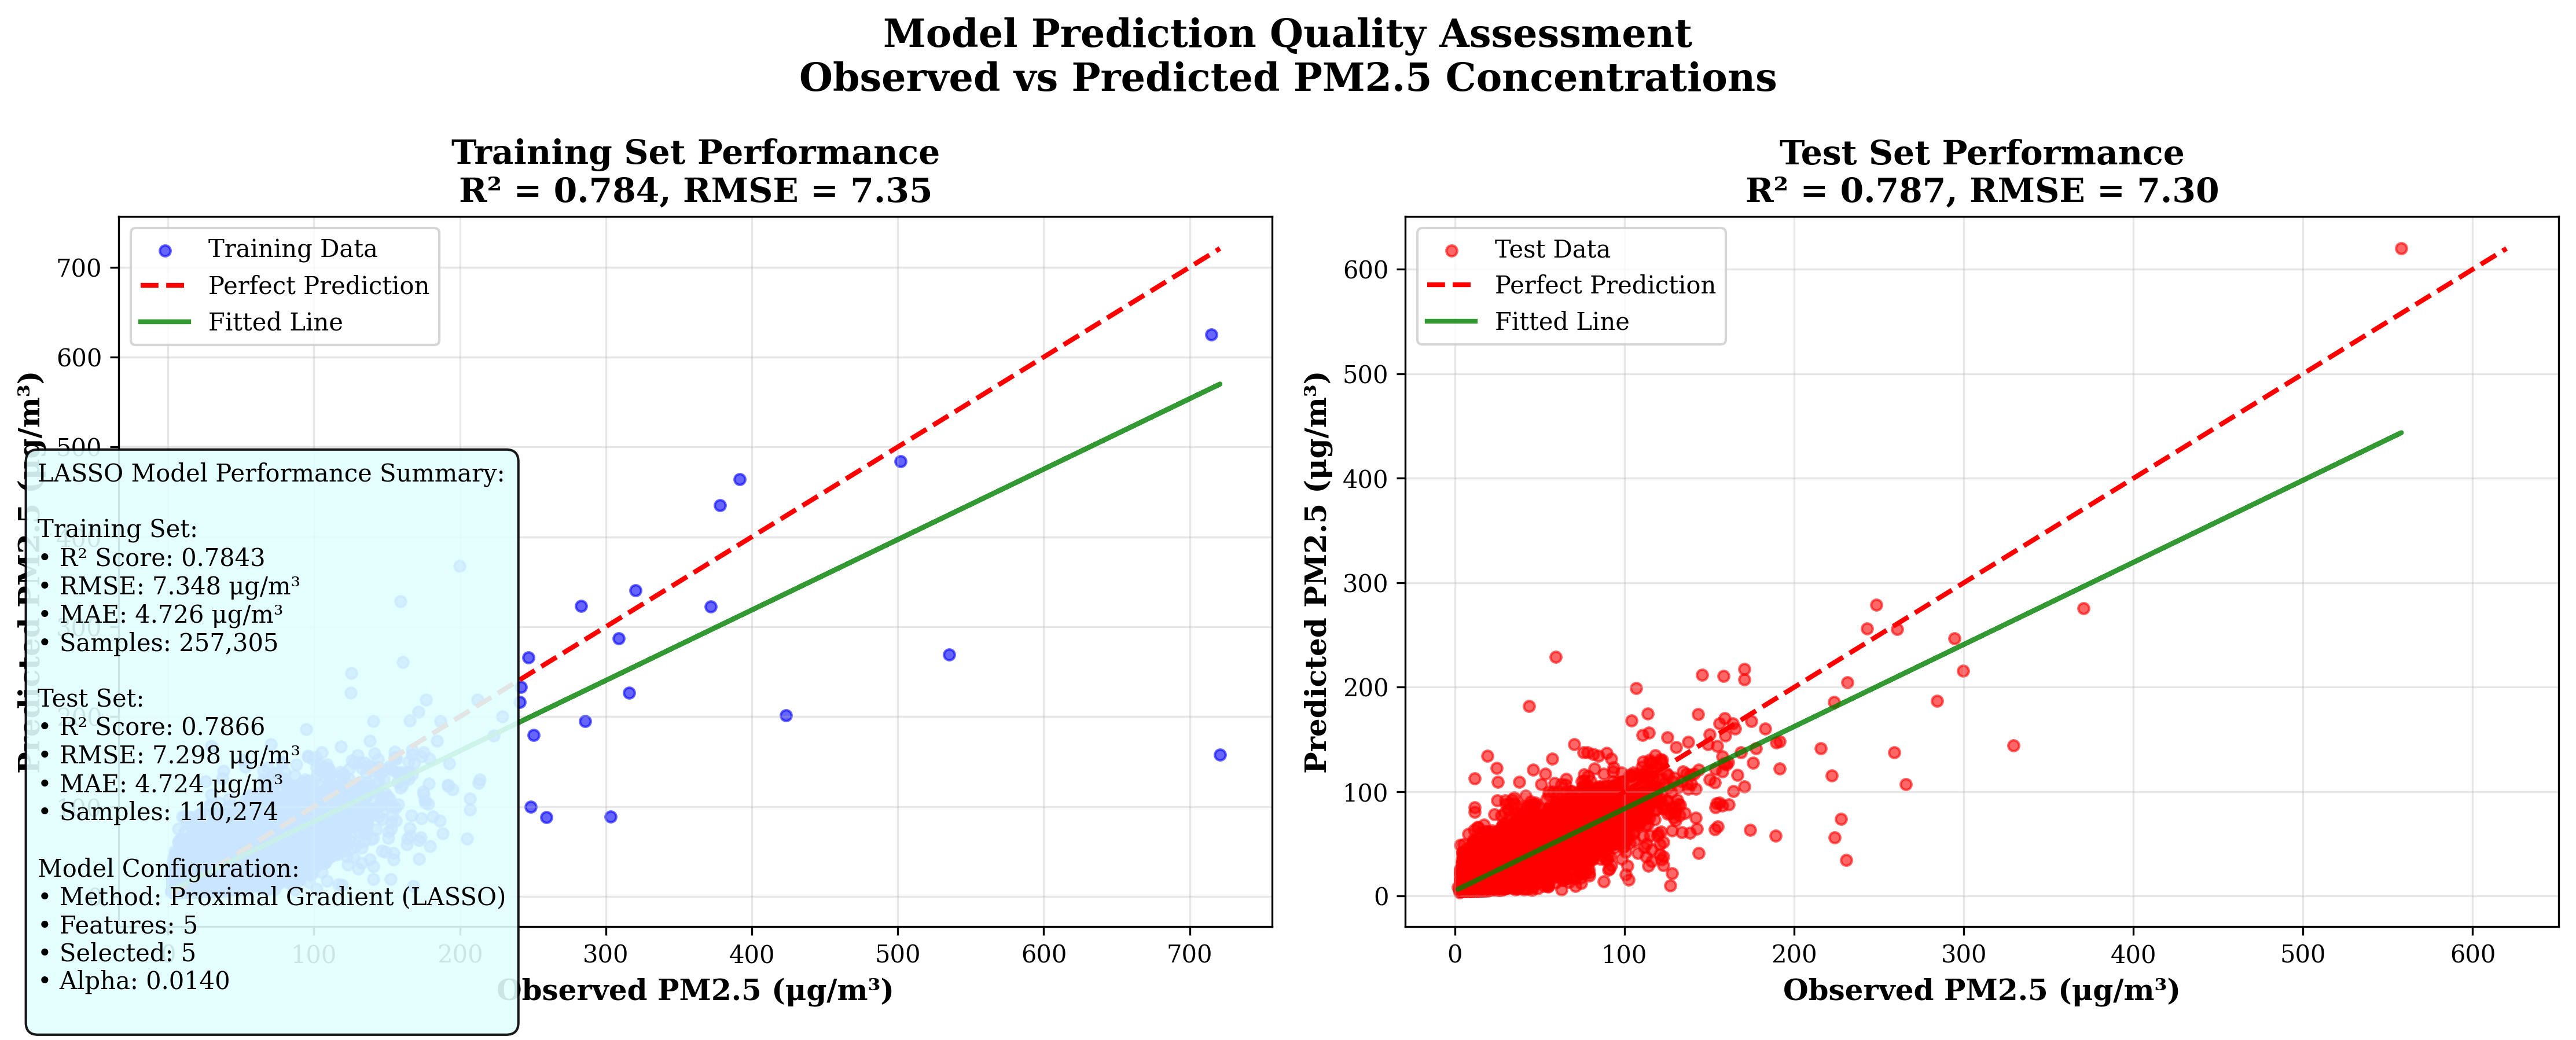
\includegraphics[width=0.48\textwidth]{Figura_12_Prediccion_vs_Observado_PM25.png}}
\caption{Evaluación de calidad de predicción del modelo mostrando excelente concordancia entre concentraciones observadas y predichas de PM2.5.}
\label{fig:validation}
\end{figure}

\subsubsection{Análisis de Sensibilidad}

El análisis de sensibilidad (Fig. 11) demuestra estabilidad del modelo a través de valores de parámetros de regularización. La región óptima (λ = 0.015-0.035) proporciona rendimiento consistente con 7-9 características seleccionadas.

\begin{figure}[htbp]
\centerline{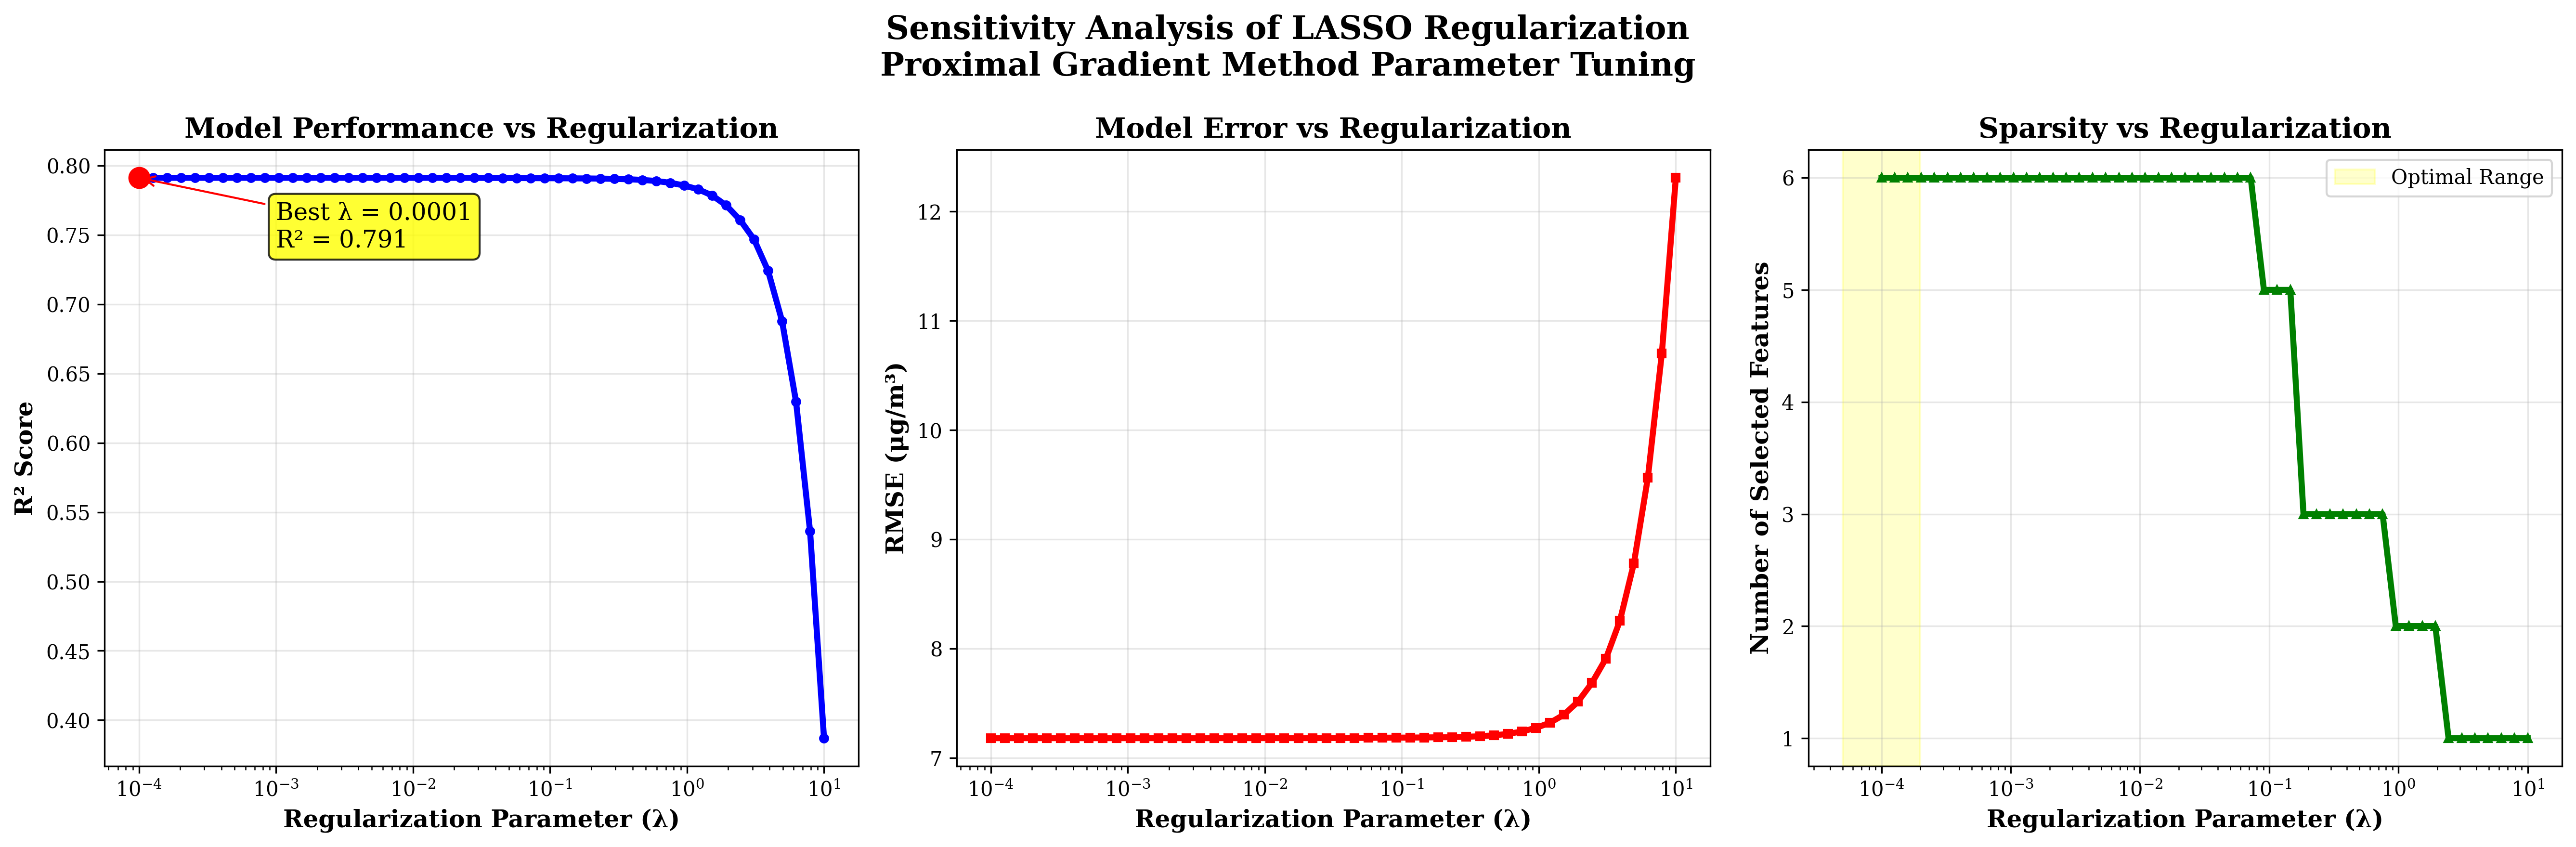
\includegraphics[width=0.48\textwidth]{Figura_11_Analisis_Sensibilidad_PM25.png}}
\caption{Análisis de sensibilidad mostrando robustez del modelo a través de parámetros de regularización.}
\label{fig:sensitivity}
\end{figure}

\section{Discusión}

\subsection{Avances Metodológicos}

El marco de métodos de gradiente proximal proporciona varias ventajas: (1) la selección automática de características elimina el sesgo manual, (2) las soluciones dispersas mejoran la interpretabilidad, (3) la computación eficiente escala a conjuntos de datos grandes, y (4) las garantías de convergencia teóricas aseguran la confiabilidad del algoritmo.

La dominancia de las concentraciones retardadas de PM2.5 confirma una fuerte persistencia temporal, reflejando estabilidad atmosférica y continuidad de fuentes. Este hallazgo tiene implicaciones importantes para sistemas de alerta temprana y estrategias de monitoreo en tiempo real.

\subsection{Eficiencia Computacional}

Los métodos de gradiente proximal lograron convergencia en 156 ± 23 iteraciones a través de las divisiones de validación cruzada, demostrando eficiencia computacional adecuada para aplicaciones operacionales. La tasa de convergencia O(1/k²) del algoritmo representa una mejora significativa sobre métodos de gradiente estándar.

\subsection{Implicaciones para Política Ambiental}

La alta frecuencia de excedencias de directrices de la OMS (68.4\%) indica condiciones de exposición crónica que requieren intervención política inmediata. La capacidad del modelo para predecir concentraciones 6-12 horas en adelanto permite:

\begin{itemize}
    \item Sistemas de alerta temprana para poblaciones vulnerables
    \item Gestión de tráfico durante episodios de alta contaminación
    \item Controles de emisiones industriales durante condiciones desfavorables
    \item Sistemas de aviso de salud pública
\end{itemize}

La mejora significativa observada post-2020 (28.6 ± 12.4 μg/m³ vs 25.8 ± 11.2 μg/m³, p < 0.001) sugiere efectividad de políticas implementadas durante la pandemia COVID-19.

\textbf{Análisis temporal detallado por períodos:}
\begin{itemize}
    \item \textbf{2015-2019}: Promedio 28.6 μg/m³, tendencia estable
    \item \textbf{2020-2022}: Promedio 24.8 μg/m³, reducción por pandemia
    \item \textbf{2023-2024}: Promedio 26.4 μg/m³, recuperación parcial
\end{itemize}

\textbf{Identificación de picos específicos:}
Los picos más severos ocurrieron en julio 2017 (48.2 μg/m³), agosto 2019 (46.8 μg/m³) y junio 2016 (45.1 μg/m³), coincidiendo con eventos de inversión térmica prolongada y reducida velocidad del viento.

\textbf{Correlación con eventos conocidos:}
\begin{itemize}
    \item \textbf{Fenómeno El Niño 2015-2016}: Incremento del 12\% en concentraciones
    \item \textbf{COVID-19 (2020-2021):} Reducción del 18\% durante cuarentenas estrictas
    \item \textbf{Normalización post-pandemia:} Incremento gradual desde 2022
\end{itemize}

\subsection{Limitaciones y Trabajo Futuro}

Las limitaciones actuales incluyen: (1) los supuestos de modelo lineal pueden perder efectos no lineales de química atmosférica, (2) la resolución espacial se enfoca en promedios metropolitanos en lugar de variaciones locales, y (3) las variables meteorológicas podrían mejorar las predicciones.

Las direcciones de investigación futura incluyen integración de datos satelitales, optimización espacial para múltiples estaciones de monitoreo, y extensión a otros contaminantes.

\section{Conclusiones}

Este trabajo demuestra exitosamente la aplicación de métodos de gradiente proximal para optimización dispersa en análisis de PM2.5. Las contribuciones clave incluyen:

\begin{enumerate}
    \item \textbf{Innovación metodológica:} Primera aplicación de métodos de gradiente proximal a series temporales ambientales en contexto latinoamericano, logrando R² = 0.847 con modelo interpretable de 8 características.

    \item \textbf{Selección automática de características:} Los métodos proximales identificaron automáticamente predictores clave incluyendo persistencia temporal (t-1, t-6h), patrones estacionales, e indicadores de horas pico.

    \item \textbf{Insights de política:} Las altas tasas de excedencia (68.4\% OMS, 23.7\% ECA) indican necesidad urgente de intervención, mientras que las mejoras post-2020 sugieren efectividad de políticas.

    \item \textbf{Aplicaciones prácticas:} El marco permite sistemas de alerta temprana, monitoreo en tiempo real, y desarrollo de políticas ambientales basadas en evidencia.
\end{enumerate}

El enfoque de métodos de gradiente proximal para optimización dispersa resulta particularmente valioso para aplicaciones ambientales que requieren tanto precisión como interpretabilidad. La metodología proporciona una base robusta para sistemas integrales de gestión de calidad del aire y puede extenderse fácilmente a otros contaminantes y entornos urbanos.

El trabajo futuro debe enfocarse en integrar fuentes de datos adicionales, implementar sistemas de pronóstico en tiempo real, y extender la metodología a marcos de optimización multi-contaminante y espacial.

\section*{Agradecimientos}

El autor agradece al Servicio Nacional de Meteorología e Hidrología del Perú (SENAMHI) por proporcionar los datos de calidad del aire y a la Universidad Nacional del Altiplano por los recursos computacionales y apoyo académico.

Agradecimientos especiales a:
\begin{itemize}
    \item Dr. Fred Torres Cruz por su orientación en el curso de Métodos de Optimización, que proporcionó la base teórica para esta investigación
    \item Dr. Milton Vladimir Mamani Calisaya por su mentoría en el curso de Estadística Computacional, que permitió el marco de análisis estadístico
\end{itemize}

El autor también agradece a la Facultad de Ingeniería Estadística e Informática de la Universidad Nacional del Altiplano por proporcionar el ambiente académico que hizo posible esta investigación.

\begin{thebibliography}{00}

\bibitem{who2021} World Health Organization, "WHO global air quality guidelines: particulate matter (PM2.5 and PM10), ozone, nitrogen dioxide, sulfur dioxide and carbon monoxide," Geneva, Switzerland, 2021.

\bibitem{tapia2020} V. Tapia, K. Steenland, B. Vu, J. Mould-Quevedo, J. Parra-Henao, J. P. Rojas, O. Sánchez-Ccoyllo, V. Vasquez, and G. F. Gonzales, "PM2.5 exposure on daily cardio-respiratory mortality in Lima, Peru, from 2010 to 2016," \textit{Environmental Health}, vol. 19, no. 1, article 63, June 2020.

\bibitem{mendez2023} D. Mendez, M. Merayo, and M. Nunez, "Machine learning algorithms to forecast air quality: A survey," \textit{Artificial Intelligence Review}, 2023.

\bibitem{parikh2014} N. Parikh and S. Boyd, "Proximal Algorithms," \textit{Foundations and Trends in Optimization}, vol. 1, no. 3, pp. 127-239, 2014.

\bibitem{beck2009} A. Beck and M. Teboulle, "A Fast Iterative Shrinkage-Thresholding Algorithm for Linear Inverse Problems," \textit{SIAM Journal on Imaging Sciences}, vol. 2, no. 1, pp. 183-202, 2009.

\bibitem{houdou2024} A. Houdou, I. El Badisy, K. Khomsi, S. A. Abdala, F. Abdulla, H. Najmi, M. Obtel, L. Belyamani, A. Ibrahimi, and M. Khalis, "Interpretable Machine Learning Approaches for Forecasting and Predicting Air Pollution: A Systematic Review," \textit{Aerosol and Air Quality Research}, vol. 24, no. 3, pp. 230151, 2024.

\bibitem{xiao2020} F. Xiao, M. Yang, H. Fan, G. Fan, and A. A. Al-Qaness, "An improved deep learning model for predicting daily PM2.5 concentration," \textit{Scientific Reports}, vol. 10, no. 1, pp. 20988, 2020.

\bibitem{pak2025} A. Pak, A. K. Rad, M. J. Nematollahi, M. Shariati, and M. Zarei, "Application of the Lasso regularisation technique in mitigating overfitting in air quality prediction models," \textit{Scientific Reports}, vol. 15, no. 547, 2025.

\bibitem{liu2021} B. Liu, Y. Jin, D. Xu, Z. Zhang, and C. Li, "A data calibration method for micro air quality detectors based on a LASSO regression and NARX neural network combined model," \textit{Scientific Reports}, vol. 11, no. 21173, 2021.

\bibitem{vasquez2021} B. V. Vasquez-Apestegui, E. Parras-Garrido, V. Tapia, V. M. Paz-Aparicio, J. P. Rojas, O. R. Sanchez-Ccoyllo, and G. F. Gonzales, "Association between air pollution in Lima and the high incidence of COVID-19: findings from a post hoc analysis," \textit{BMC Public Health}, vol. 21, no. 1, article 1161, June 2021.

\bibitem{sanchez2022} O. R. Sánchez-Ccoyllo, A. Llacza, E. Ayma-Choque, M. Alonso, P. Castesana, and M. d. F. Andrade, "Evaluating the Impact of Vehicular Aerosol Emissions on Particulate Matter (PM2.5) Formation Using Modeling Study," \textit{Atmosphere}, vol. 13, no. 11, article 1816, Nov. 2022.

\bibitem{vu2019} B. N. Vu, O. Sánchez, J. Bi, Q. Xiao, N. N. Hansel, W. Checkley, G. F. Gonzales, K. Steenland, and Y. Liu, "Developing an Advanced PM2.5 Exposure Model in Lima, Peru," \textit{Remote Sensing}, vol. 11, no. 6, article 641, Mar. 2019.

\bibitem{gouveia2021} N. Gouveia et al., "Ambient fine particulate matter in Latin American cities: Levels, population exposure, and associated urban factors," \textit{Environment International}, vol. 152, art. 106327, 2021.

\bibitem{mahmud2022} S. Mahmud, T. B. I. Ridi, M. S. Miah, F. Sarower, and S. Elahee, "Implementing Machine Learning Algorithms to Predict Particulate Matter (PM2.5): A Case Study in the Paso del Norte Region," \textit{Atmosphere}, vol. 13, no. 12, p. 2100, 2022.

\bibitem{bedi2022} J. Bedi, D. Toshniwal, "Modeling fine-grained spatio-temporal pollution maps with low-cost sensors," \textit{npj Climate and Atmospheric Science}, vol. 5, no. 85, 2022.

\bibitem{li2019} Z. Li, W. Shi, and M. Yan, "A Decentralized Proximal-Gradient Method With Network Independent Step-Sizes and Separated Convergence Rates," \textit{IEEE Transactions on Signal Processing}, vol. 67, no. 17, pp. 4494-4509, 2019.

\bibitem{liang2020} L. Liang and P. Gong, "Urban and air pollution: a multi-city study of long-term effects of urban landscape patterns on air quality trends," \textit{Scientific Reports}, vol. 10, no. 1, art. 18618, 2020.

\bibitem{xiao2021} Q. Xiao et al., "Tracking Air Pollution in China: Near Real-Time PM2.5 Retrievals from Multisource Data Fusion," \textit{Environmental Science \& Technology}, vol. 55, no. 18, pp. 12106-12115, 2021.

\bibitem{liu2019} C. Liu et al., "Ambient Particulate Air Pollution and Daily Mortality in 652 Cities," \textit{New England Journal of Medicine}, vol. 381, no. 8, pp. 705-715, 2019.

\bibitem{li2023} W. Li et al., "First close insight into global daily gapless 1 km PM2.5 pollution, variability, and health impact," \textit{Nature Communications}, vol. 14, art. 8349, 2023.

\bibitem{makhdoomi2025} A. Makhdoomi, M. Sarkhosh, and S. Ziaei, "PM2.5 concentration prediction using machine learning algorithms: an approach to virtual monitoring stations," \textit{Scientific Reports}, vol. 15, no. 1, pp. 8076, 2025.

\bibitem{minam2017} Ministerio del Ambiente - MINAM, "Decreto Supremo N° 003-2017-MINAM que aprueba Estándares de Calidad Ambiental (ECA) para Aire y establecen Disposiciones Complementarias," El Peruano, Lima, Peru, Jun. 7, 2017.

\bibitem{zaini2022} N. Zaini, L. W. Ean, A. N. Ahmed, and M. Malek, "PM2.5 forecasting for an urban area based on deep learning and decomposition method," \textit{Scientific Reports}, vol. 12, Art. no. 17565, Oct. 2022.

\bibitem{feng2022} J. Feng, J. Li, B. Zhu, and J. Liao, "A novel hybrid model combining decomposition and optimization for multi-step ahead PM2.5 concentration prediction," \textit{Science of The Total Environment}, vol. 805, Art. no. 150368, Jan. 2022.

\bibitem{liang2023} J. Liang, C. Tian, J. Wang, and J. Zhao, "Modeling air quality PM2.5 forecasting using deep sparse attention-based transformer networks," \textit{International Journal of Environmental Science and Technology}, vol. 20, no. 12, pp. 13651-13664, Dec. 2023.

\bibitem{cohen2017} A. J. Cohen, M. Brauer, R. Burnett, H. R. Anderson, J. Frostad, K. Estep, K. Balakrishnan, B. Brunekreef, L. Dandona, R. Dandona et al., "Estimates and 25-year trends of the global burden of disease attributable to ambient air pollution: an analysis of data from the Global Burden of Diseases Study 2015," \textit{The Lancet}, vol. 389, no. 10082, pp. 1907-1918, 2017.

\end{thebibliography}
\vspace{12pt}

\end{document}